\normallinespacing

\chapter{Methods}
This projects follows a mixed-methods approach to answer the research questions. For this purpose, methodological triangulation is used by involving different methods and/or types of data to study the same research question. If the results and evidence from different types of data are in agreement, they help in validating the finding of each\cite{fraenkel_wallen_hyun_2019}. Quantitative and qualitative data are used and given the same hierarchy to assess orchestration load and usability of the PyramidApp dashboard. This section describes the data collection methods employed for this project and the analysis conducted with it.
\begin{figure}[!h]
    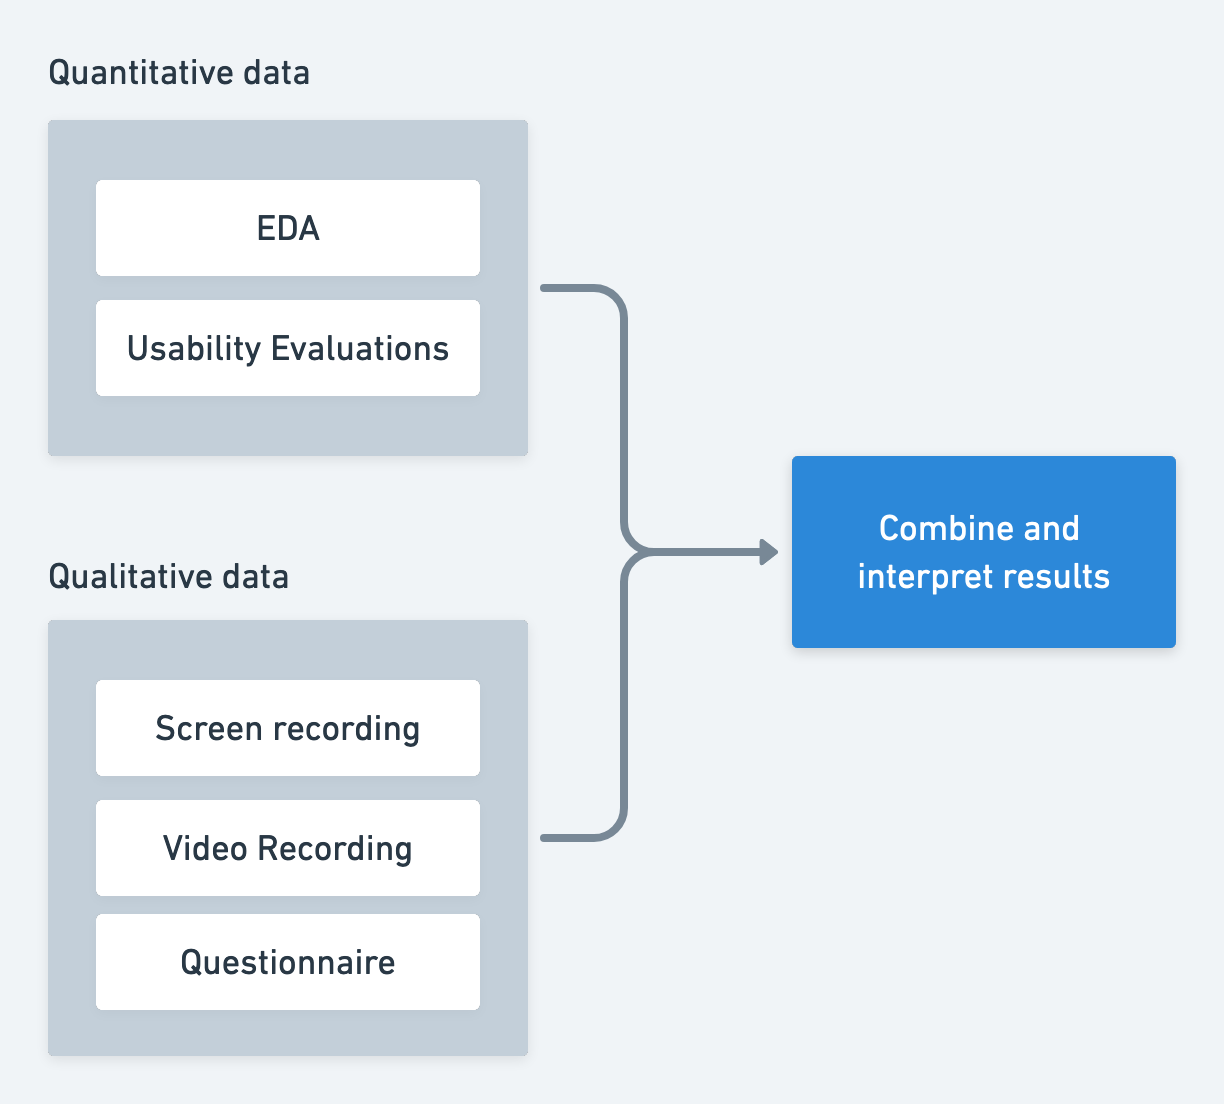
\includegraphics[clip,width=\columnwidth]{Figures/triangulation.png}% 
\caption{Methodological triangulation as described by Fraenkel (2011)}
\label{fig:triangulation}
\end{figure}
\section{Participants}
In order to answer the research questions, a purposive type of sampling was used to reach subjects that participated in the experiments. This section describes the sampling method selected, the target population and the accessible population that were reached for the data collection.
\subsection{Sampling}
Even though selecting participants through a random sampling is optimal for research purposes \cite{fraenkel_wallen_hyun_2019}, due to the resource limitations of this project and the current adoption of PyramidApp, this was not an option. There were not enough accessible teachers that met the selection criteria to create a pool of potential participants from where to randomly draw for the data collection. This being the main limitation, a purposive sampling approach was used to select participants. The researcher used their judgement to select a sample that they believed, based on prior information, would provide the data needed to answer the research questions proposed in this thesis \cite{fraenkel_wallen_hyun_2019}. The main criteria to select the sample was having previous teaching experience and experience using PyramidApp. The reason for this, was the avoidance of the novelty effect, that is, the phenomenon in which individuals might perceive or respond differently to a novel situation than they would in a common, familiar context \cite{gravetter_2016}.
\subsection{Population}
The population to which this project aims to generalise are university teachers who impart classes online in real time, who are familiarised with moderating CSCL activities and the usage of teacher dashboards. \\To represent this population, a male and a female teachers from a Spanish university were recruited to participate in the data collection. They both have over 3 years imparting classes and had previous experience authoring and moderating CSCL activities.
\section{Environment} \label{environment}
Due to the equipment needed for the data collection, each participant was required to be present at a university, in a room prepared for the data collection. The room was equipped with a desk, chair and high-speed internet connection. The environment was neutral and had natural light coming from a windowed wall. Occasional street noises could be heard.\\ For each session, after the recording equipment (described later in \ref{recording-equipment}) was set up by the researcher, the participant was left alone in the room for them to impart class as they would do normally. When the class finished, the participant would let the researcher know, who would then enter the room and dismount the equipment.
\section{Materials}
\subsection{PyramidApp} \label{intro-pyramidapp}
As previously mentioned, the software that the teachers used is PyramidApp. The following section describes the foundations and applicability of this software.\\
Collaborative Learning Flow Patterns: e.g., Collaborative Learning Flow Patterns (CLFPs) refers to broadly accepted collaboration scripts that structure the flow of collaboration \cite{hernandez-leo_villasclaras-fernandez}. Examples of CLFPs are Snowball, Thinking Aloud Pair Problem Solving (TAPPS) and Pyramid \cite{Manathunga2018-uu}. Pyramid CLFP were first introduced by Davis, 2002 \cite{Davis_undated-sg} and described by Hernández-Leo \cite{Hernandez-leo2006-lv}. In a Pyramid activity, students start at level one, where they are prompted with an initial problem to which they propose a preliminary solution. Once every student has proposed an answer, the class moves to a second level in which individual students' solutions are discussed in small groups and modified to reach a single answer per group as internal consensus. In the next level, groups from level two are merged to form larger groups to discuss again and reach consensus. This process is repeated until a consensus is reached at the class level \cite{Manathunga2018-uu}.\\
PyramidApp is a web-based software that implements a particularisation of Pyramid CLFP \cite{Manathunga2018-uu}. It is integrated within the Integrated Learning Design Environment (ILDE) \cite{ILDE}. PyramidApp is accessible at https://ilde.upf. edu/pg/lds/neweditor/pyramid/ (registration is required), and a complete manual of the tool can be found in link. The software is divided into three parts:
\subsubsection{Authoring}
The authoring of a PyramidApp activity is done in two steps. In the first step, the teacher is prompted to name a title for the activity and define the question that the students will answer. Figure \ref{fig:P1} displays the interface for this first step.
\begin{figure}[!h]
    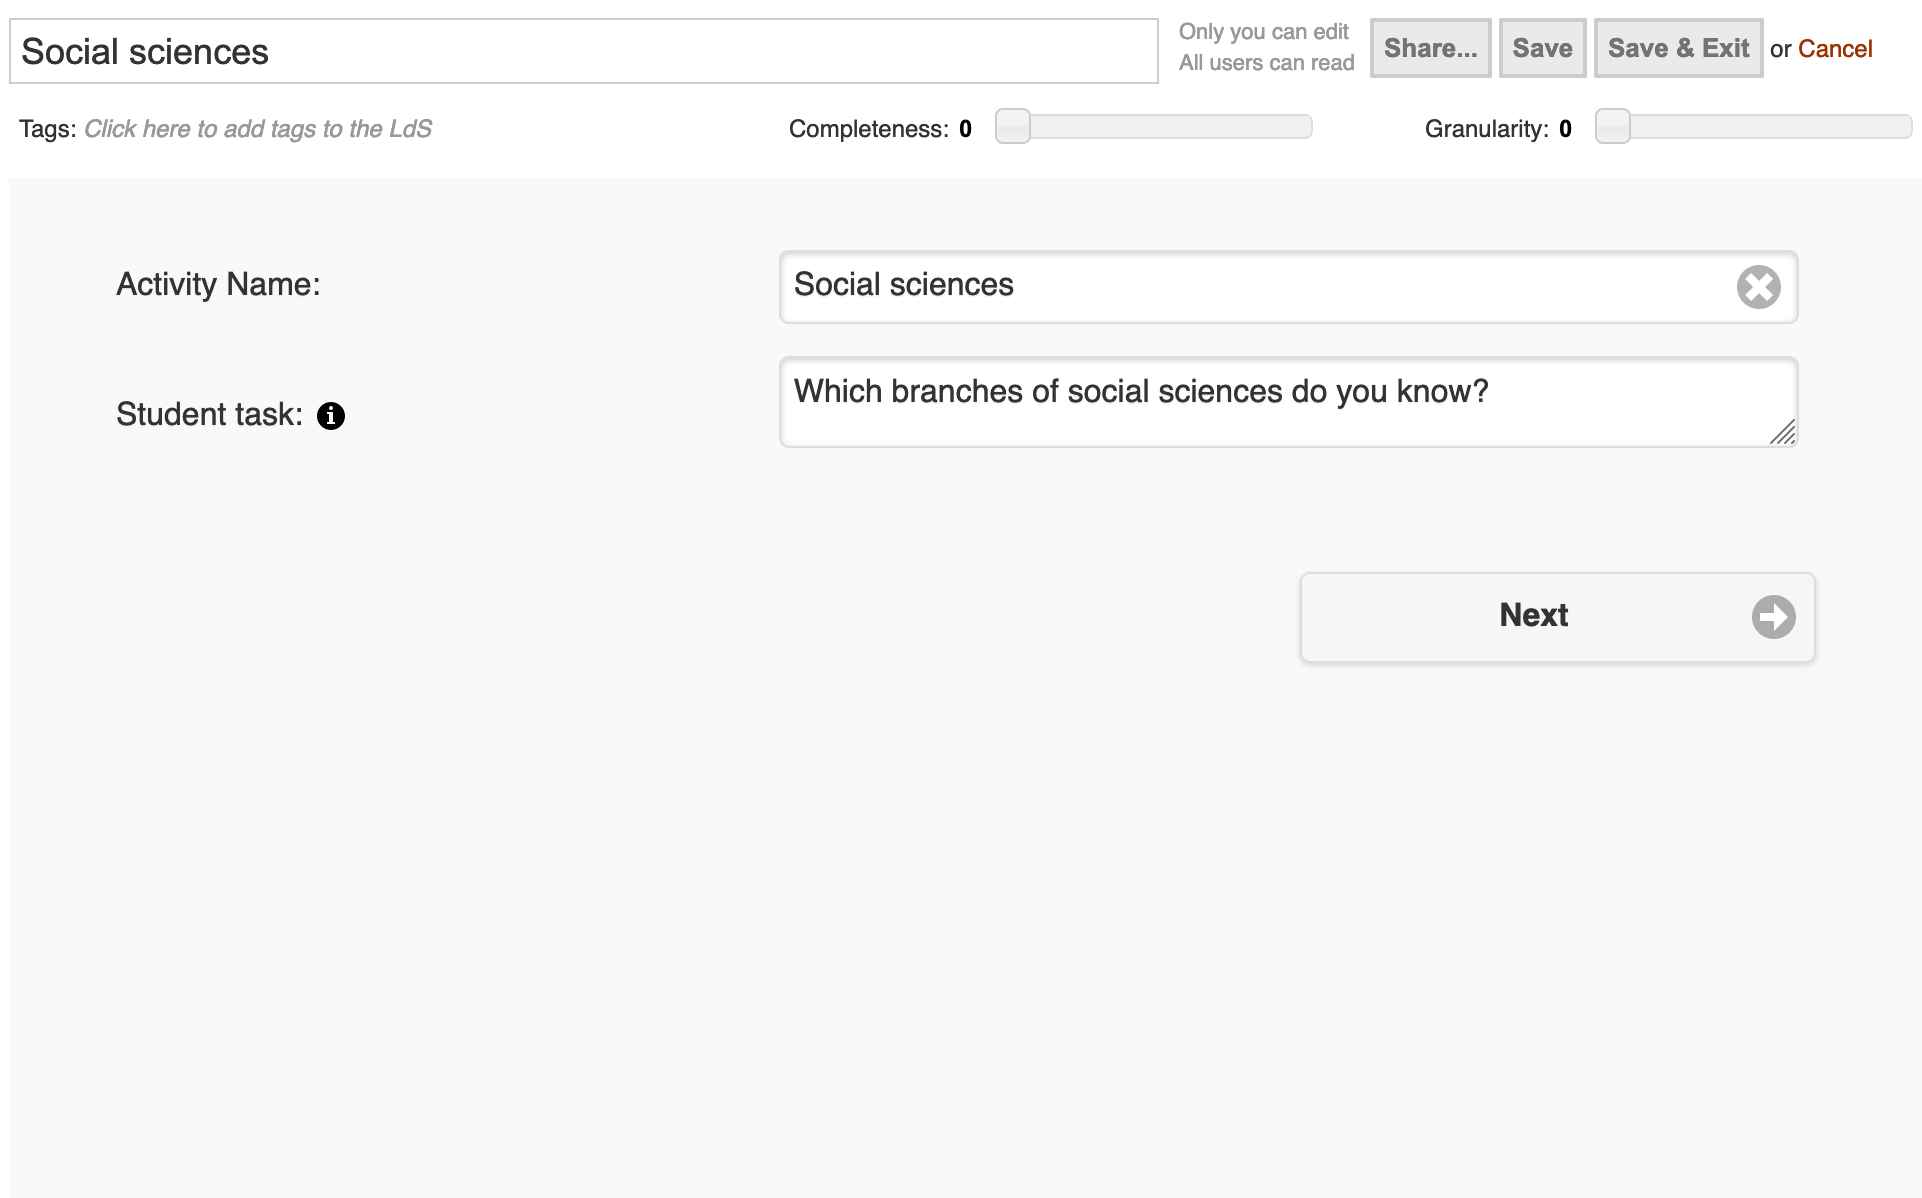
\includegraphics[clip,width=\columnwidth]{Figures/pyramidapp1.png}%  
\caption{Authoring, First step}
\label{fig:P1}
\end{figure}
In a second step (Figure \ref{fig:P2}) the author is asked to define the total number of students participating in the activity (commonly equivalent to the amount of students in class), the initial number of students per group at rating (level two as described in \ref{intro-pyramidapp}), and the total number of Pyramid levels. Level one is an individual submission stage, and the following levels are collaborative. Each user input is explained through the black information icon (tooltip) next to each prompt. On the left, a dynamic representation of the pyramid is shown as the user modifies the initial settings. Through the "Advanced Settings" button (Figure \ref{fig:P3}), time limits for each level can be set. Through "Keywords" (Figure \ref{fig:P4}) the teacher can define words that are expected to be used by students as they progress with the activity. These keywords can be then used to create alerts that should help the teacher make pedagogical decisions during the activity. Through the configuration of alerts (Figure \ref{fig:P5}), the condition of each experiment is defined (described in \ref{conditions}). Once the activity is created, the teacher is able to save the activity, and the publish it. This creates a link that is shared with the students to join the activity.
\begin{figure}[!h]
    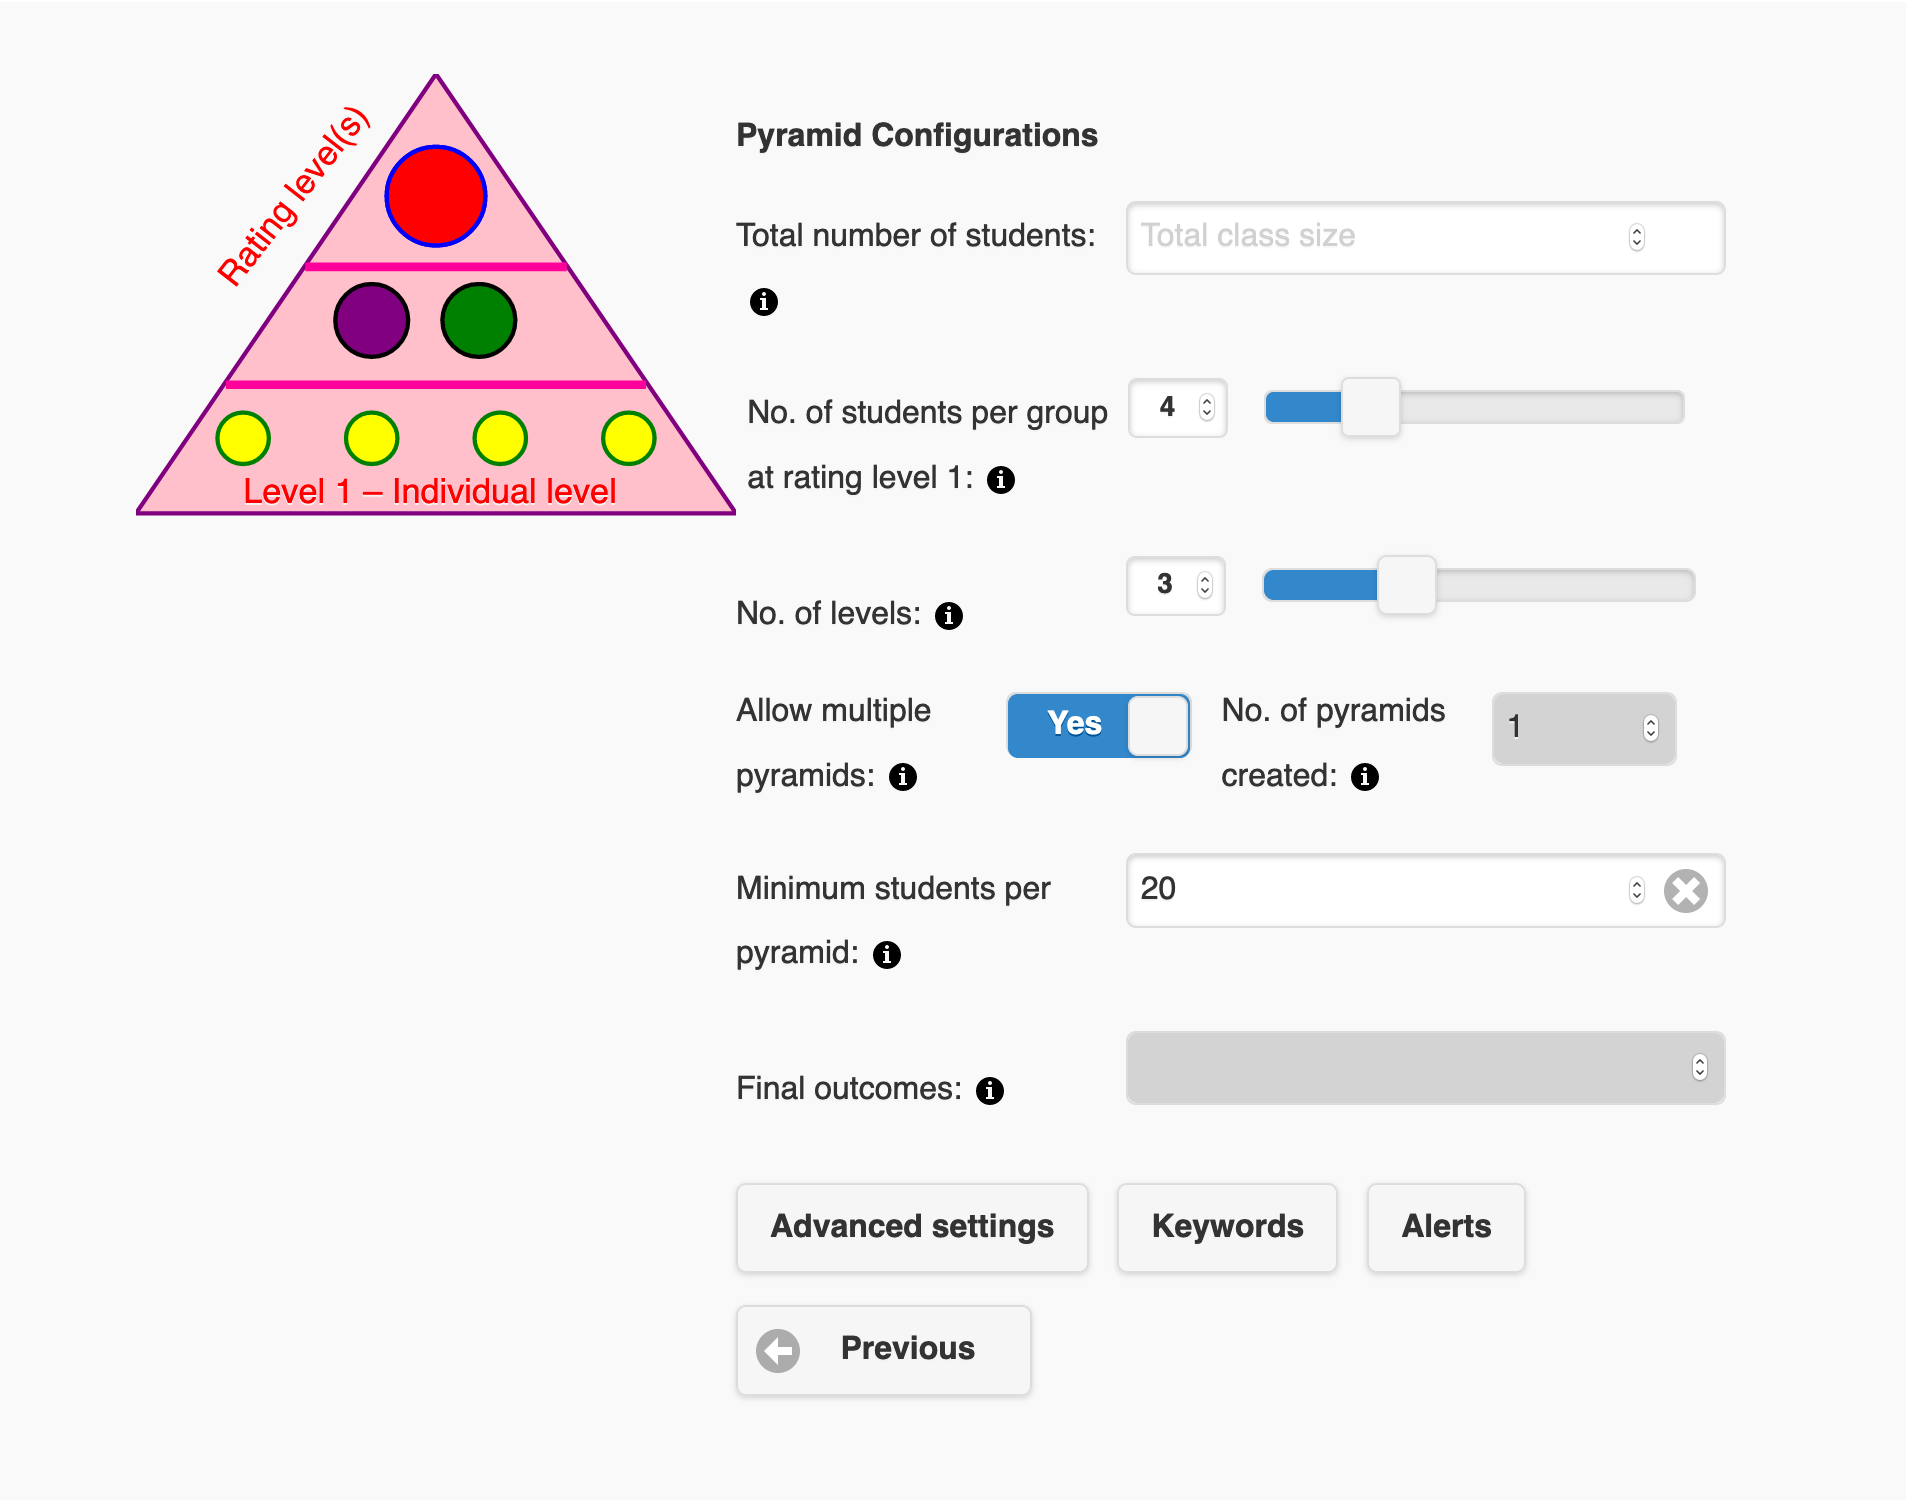
\includegraphics[clip,width=\columnwidth]{Figures/pyramidapp2.png}% 
\caption{Authoring, second step}
\label{fig:P2}
\end{figure}
\begin{figure}[!h]
    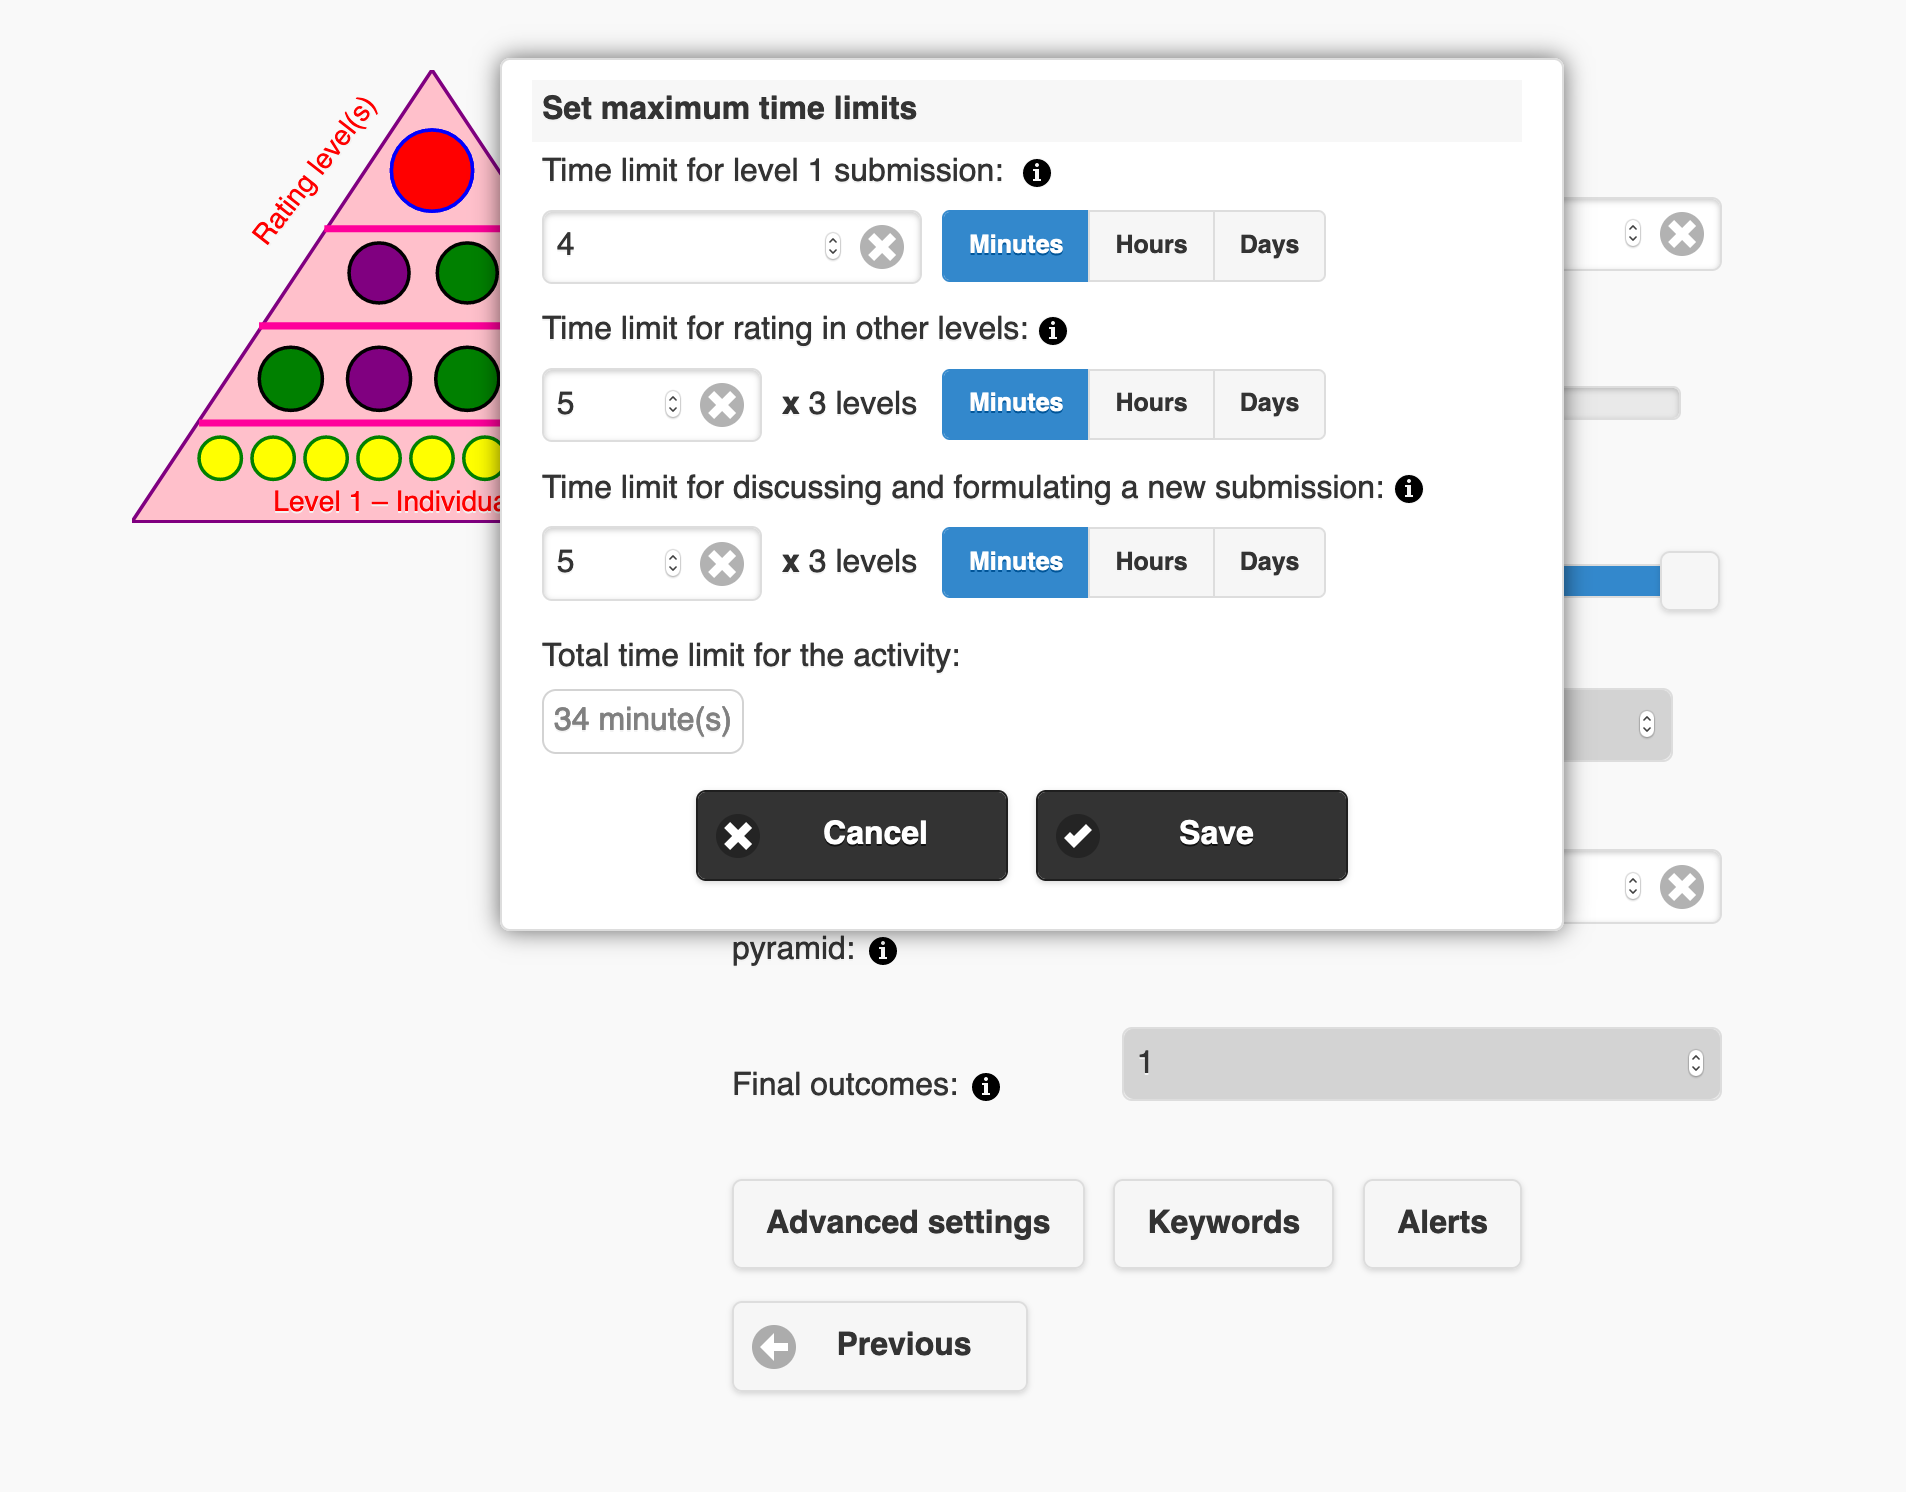
\includegraphics[clip,width=\columnwidth]{Figures/pyramidapp3.png}% 
\caption{Advanced Settings}
\label{fig:P3}
\end{figure}
\begin{figure}[!h]
    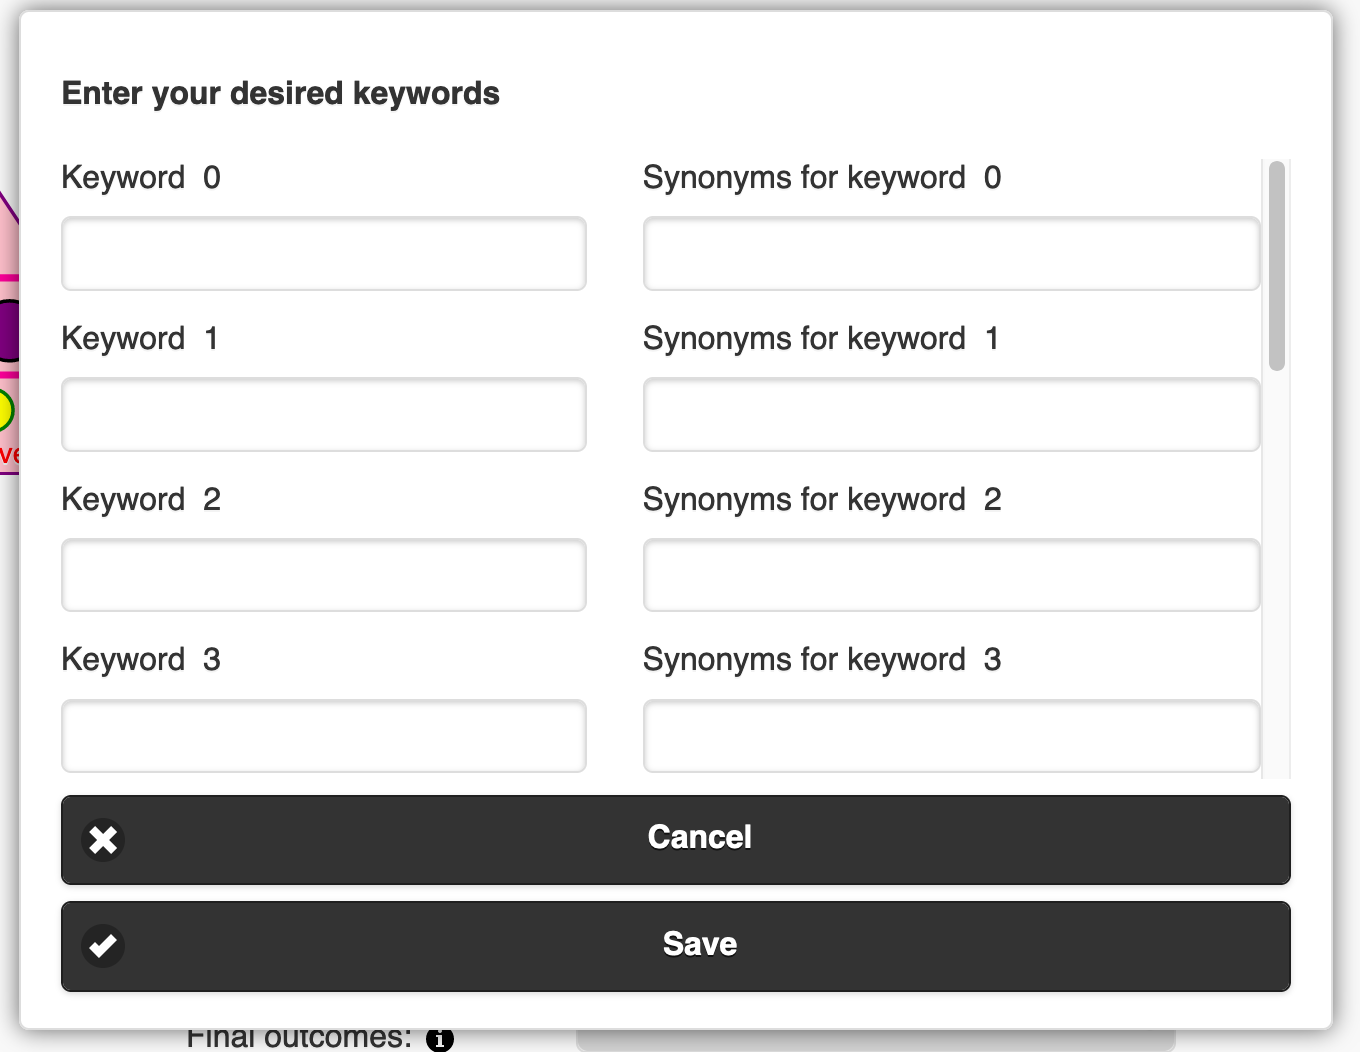
\includegraphics[clip,width=\columnwidth]{Figures/pyramidapp4.png}% 
\caption{Keyword creation}
\label{fig:P4}
\end{figure}
\begin{figure}[!h]
    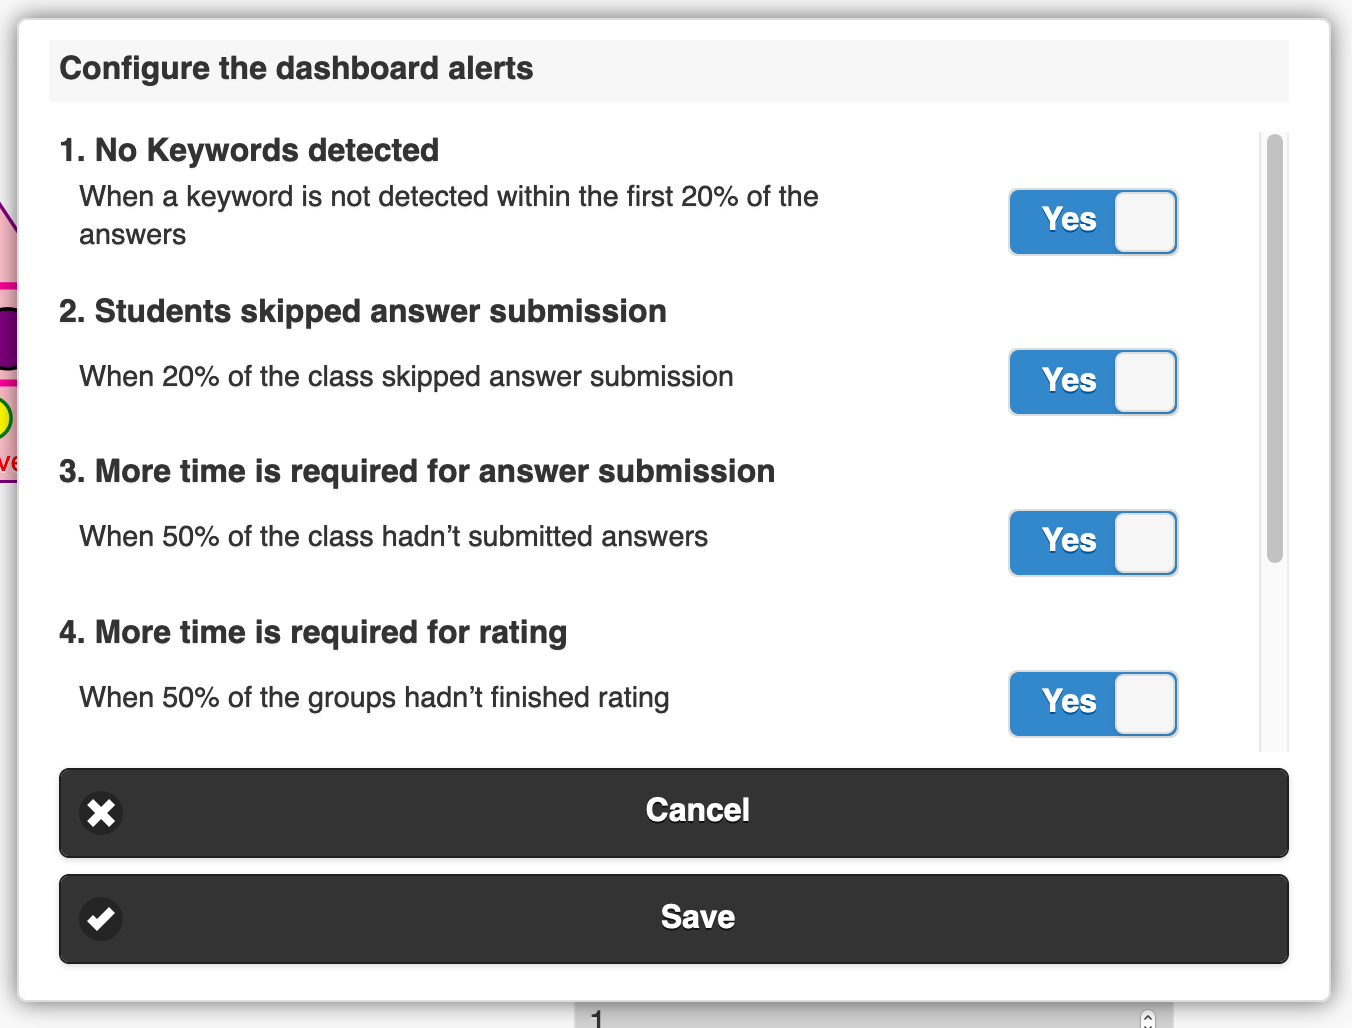
\includegraphics[clip,width=\columnwidth]{Figures/pyramidapp5.png}% 
\caption{Alert configuration}
\label{fig:P5}
\end{figure}
\subsubsection{Student's GUI}
Students enter the PyramidApp activity through the link shared by the teacher. Once a student enters, they first log in creating a username (Figure \ref{fig:P6}). Once logged in, each student will go through the levels as defined by the teacher. As shown in \ref{fig:P7}, the student will submit an initial answer to the given question. In the following levels they will collaborate with their peers either rating the submissions of other students in their group, or co-creating new submissions using a collaborative text editor. Once a class-level consensus is reached, all students see the final answer as the outcome of the activity.
\begin{figure}[!h]
    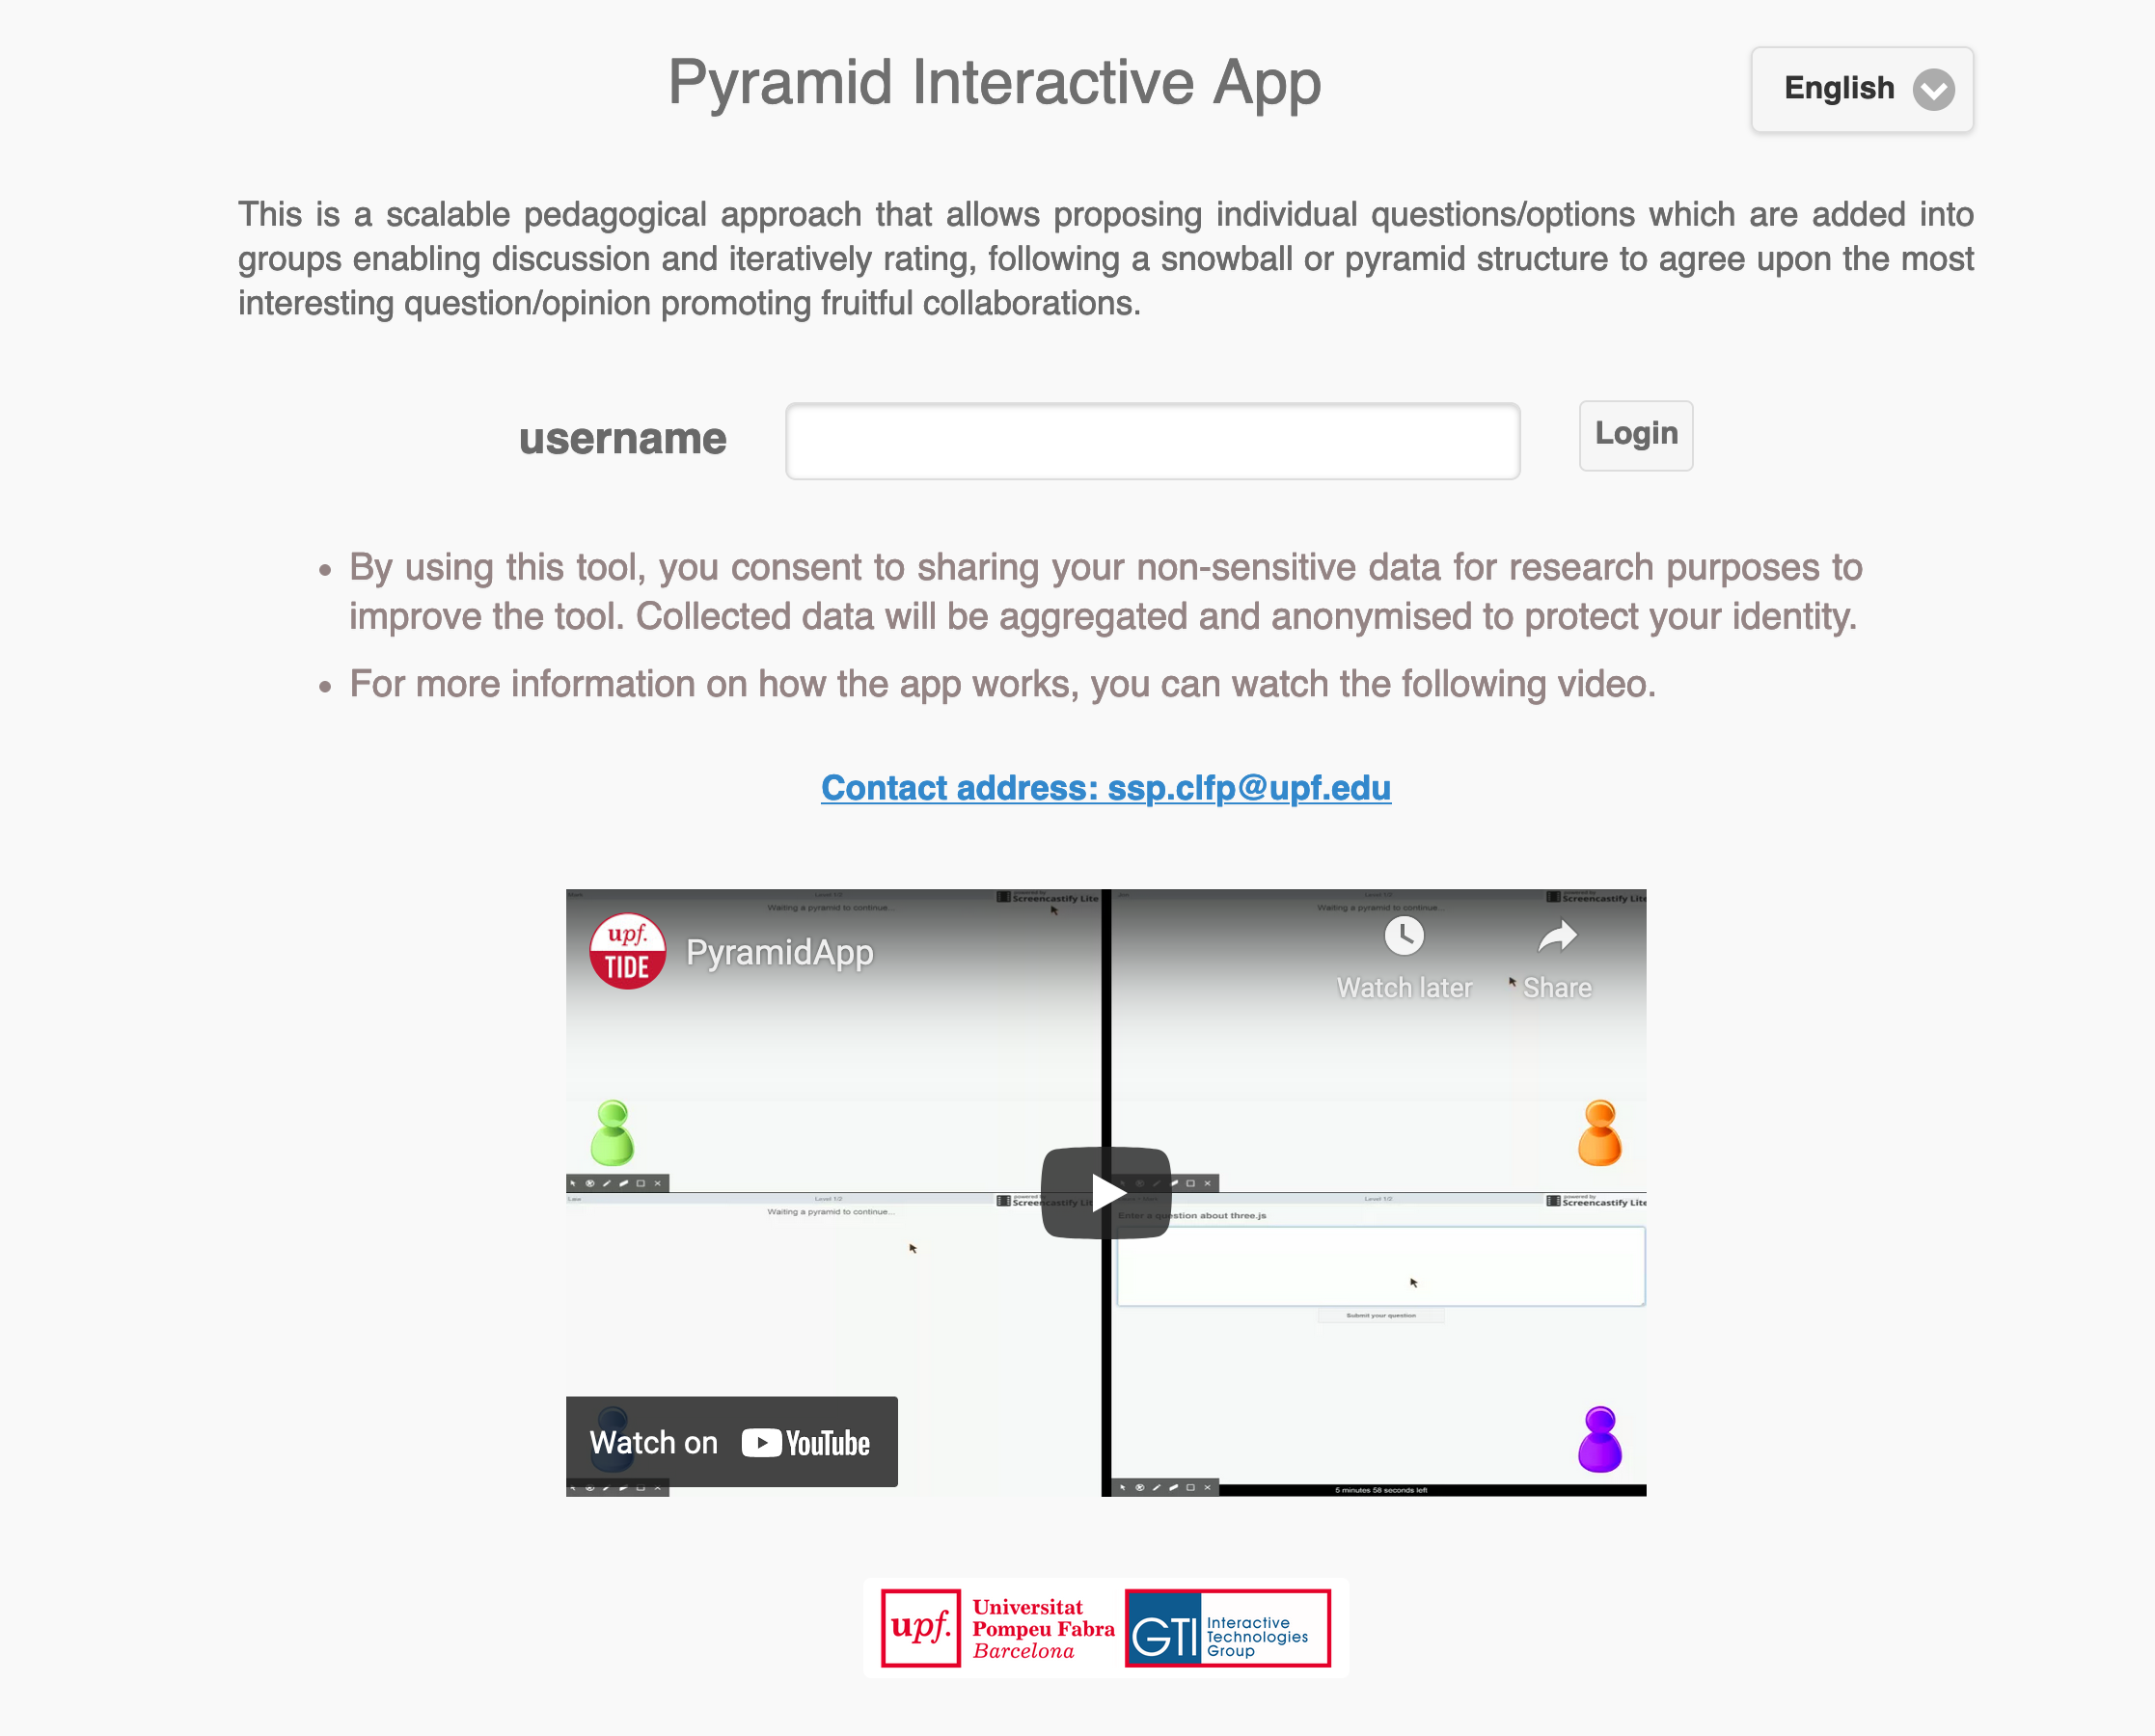
\includegraphics[clip,width=\columnwidth]{Figures/pyramidapp6.png}% 
\caption{Student's first view}
\label{fig:P6}
\end{figure}
\begin{figure}[!h]
    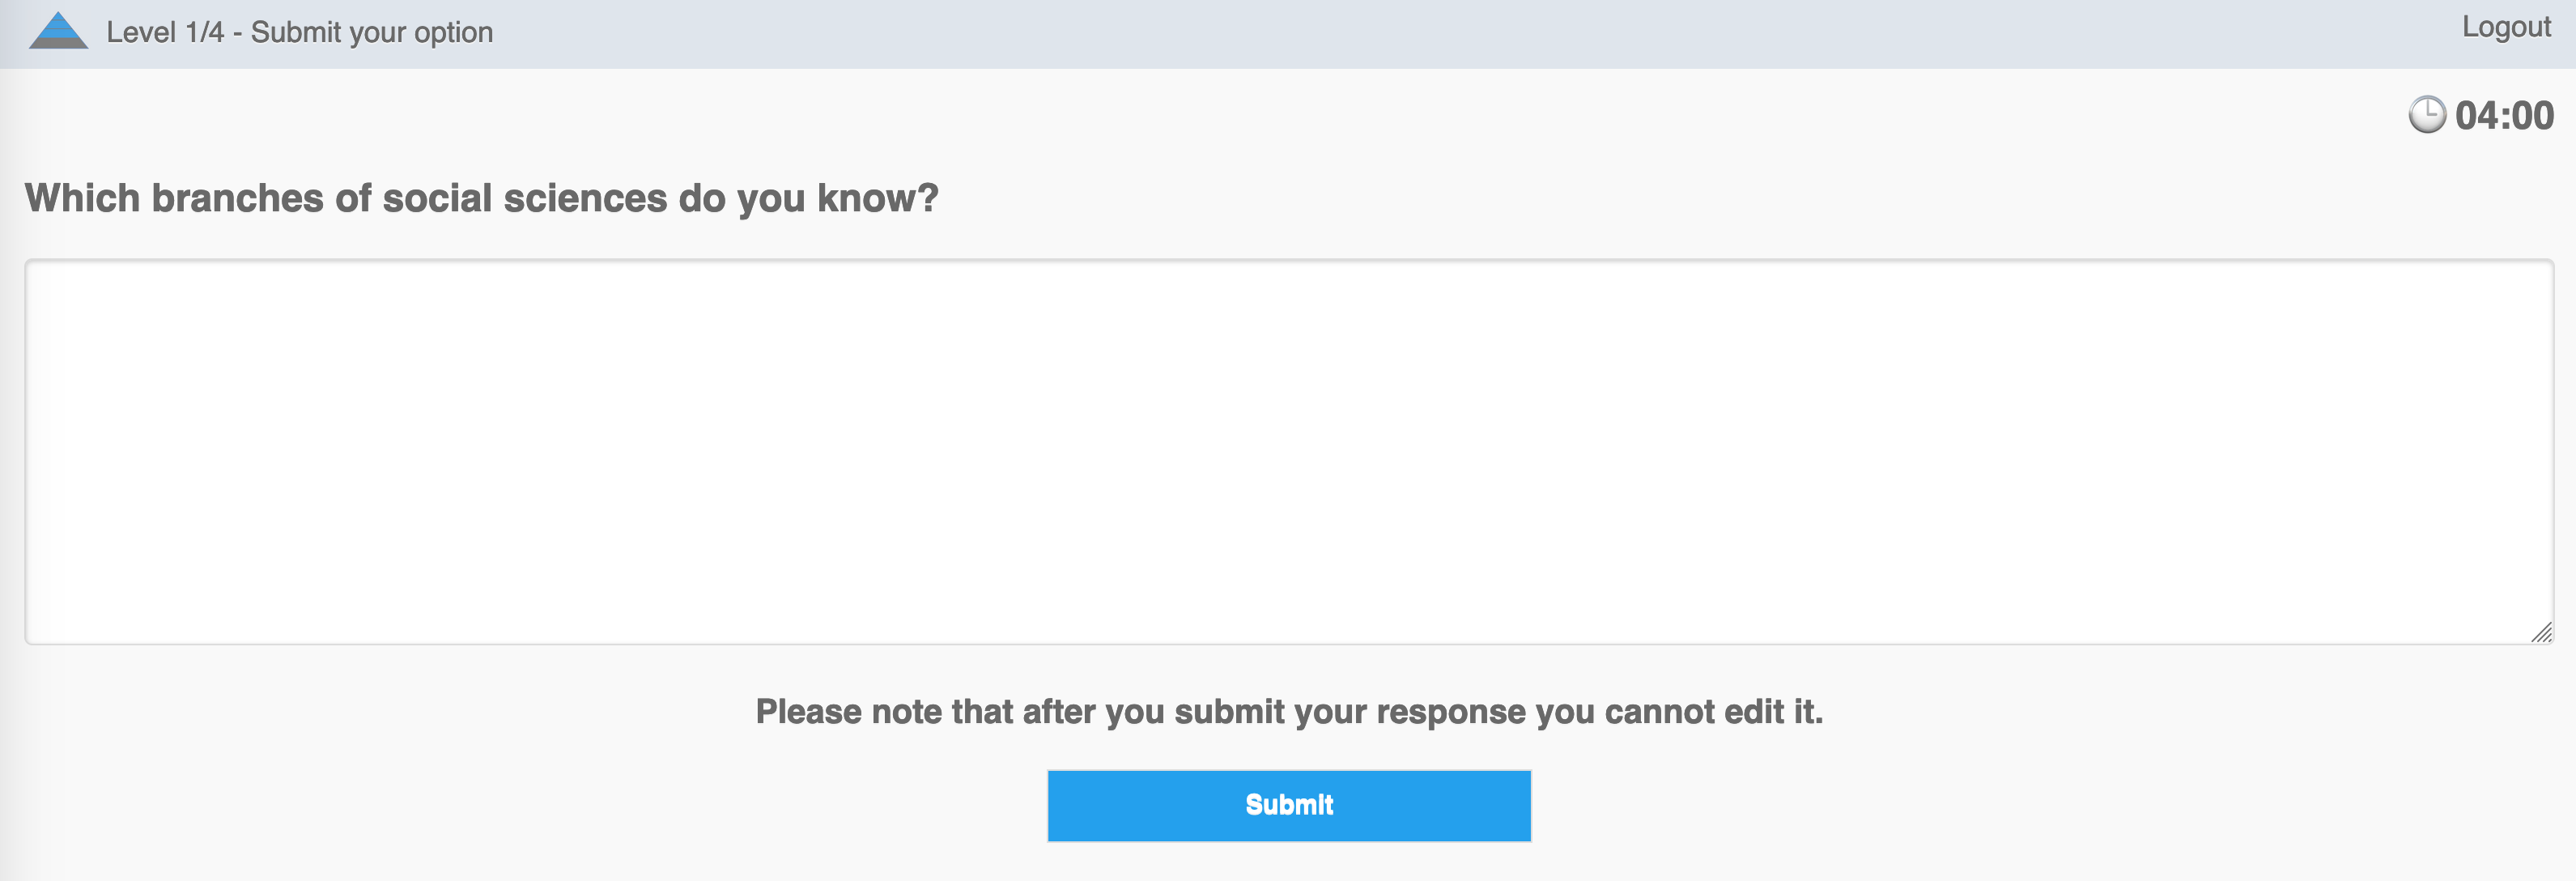
\includegraphics[clip,width=\columnwidth]{Figures/pyramidapp7.png}% 
\caption{Student's initial prompt}
\label{fig:P7}
\end{figure}

\subsubsection{Teacher Dashboard}
As the students interact with each other through PyramidApp, the teacher is shown the progress of the activity in a dashboard (Figure \ref{fig:P9}). As stated in \ref{soa_education}, dashboards are defined as a single display that aggregates multiple visualisations of different indicators about learner(s), learning process(es) and/or learning context(s). In the case of PyramidApp, the teacher is able to see the time left for the activity, current stage and upcoming stages, the amount of students connected, all options submitted and the chat logs from the students. Additionally, time and stage controls are provided for the teacher to extend time or move to the following level if necessary. Depending on the conditions described in \ref{conditions}, the teacher is helped to interpret the information presented to them in the dashboard (Figure \ref{fig:P9}). Using this information, the teacher is able to make decisions about the activity, such as providing further instructions to the students, or extending the time of the current level.

\subsection{Hardware}
The environment was equipped with a computer to run the pyramid activity. It was an Acer Aspire VX 15, with Windows 10 installed and running. All Pyramid activities were ran in Google Chrome. The operative system is important to consider given that the recording software (screen and EDA, described in \ref{recording-equipment}) may or may not be compatible with others. The computer was tested to verify that it could run PyramidApp while screen-recording without performance issues. 
The teacher was free to choose imparting the class using this computer or their own personal computer, but the pyramid activity was required to be moderated using the computer provided by the researcher. The reason for this is that the screen recording software created big-sized files and the participant might not have had enough disk space to store each file. If the computer runs out of space, it stops recording automatically which would result in the loss of key data for this project.
\section{Study Design}
\subsection{Conditions} \label{conditions}
Depending on the experimental condition, the teacher experienced the dashboard differently throughout the activity. In this project two conditions were tested. For both conditions, the teacher is presented with the student's progress through the dashboard, and has the same time and level controls over the activity. However, in the "Mirroring" condition the information presented is left for the teacher to interpret on their own, while in the "Guiding" condition alerts are displayed (Figure \ref{fig:P9}) to indicate teachers about critical situations throughout the activity. The latter is expected to provide additional support the teacher into making pedagogical decisions as they are presented with the alerts. Alerts for the guiding condition can be configured in the authoring screen (Figure \ref{fig:P5}) and are triggered in the following conditions:\\
- \textbf{No Keywords detected:} When a keyword is not detected within the first 20\% of the answers\\
- \textbf{Students skipped answer submission:} When 20\% of the class skipped answer submission\\
- \textbf{More time is required for answer submission:} When 50\% of the class hadn’t submitted answers\\
- \textbf{More time is required for rating:} When 50\% of the groups hadn’t finished rating\\
- All the groups have finished the last rating level of the activity\\
\subsection{Procedure for orchestration load data collection}
Each teacher was asked to moderate a minimum of 5 PyramidApp activities in a class with  students. The teacher was free to distribute the activities between their classes in a way that was convenient for them. The condition for the first activity was selected at random. The purpose of the first session was to introduce the students to the Pyramid flow and to PyramidApp. The following four sessions were splitted evenly between guiding and mirroring conditions. The order of the conditions was randomised. For each session electrodermal activity, screen recording, video recording and temperature were measured.
The date and time for data collection were defined weeks in advance, according to the classes in which the teacher would moderate the pyramid activity with their class. Because of this, recordings were taken at different times of the day, depending on classes and teacher availability. Teachers were free to choose the class and topic for each session. Teachers came up with the initial prompt and settings (duration, amount of students and levels) for the session. With this information, the researcher authored the activity and provided the link of the activity to the teacher. On the days in which the teachers conducted experiments, the participant went to the office reserved for the activity (described in \ref{fig:environment}). After the recording equipment was set up by the researcher (described in \ref{recording-equipment}),  the participant was left alone in the room for them to impart class as they would do normally. After each class, the researcher dismounted the equipment. At this point the teacher was prompted to complete a self-perception questionnaire (described in \ref{recording-equipment}). Data was stored in the moment for later analysis.
\subsection{Equipment for orchestration load data collection} \label{recording-equipment}
For each session, the researcher started the recording (using the software and hardware described in this section) before starting the class, and registered the time. After the session was over, the recording was stopped, time was registered again and data was stored.
\subsubsection{Dashboard Screen recording}
\textbf{Software:} Windows native recording software.
The screen of the computer was recorded while teachers engaged in the Pyramid activity. This software was chosen because of the minimal interface presented to the user while recording. It was important that the software wasn't intrusive for the participant running the experiment.
\subsubsection{Video Recording}
\textbf{Hardware:} Digital video camera Canon HD Legria HF M56 and camera tripod.
The participant was recorded in the environment throughout each class. The camera is pointed at the subject and its environment from a high angle, registering the subject in a long shot, so that their gestures are recorded (Figure \ref{fig:environment}). The camera is placed over a tripod at approximately 1.5 meters from the subject, framing the subject's right side.
\begin{figure}[!h]
    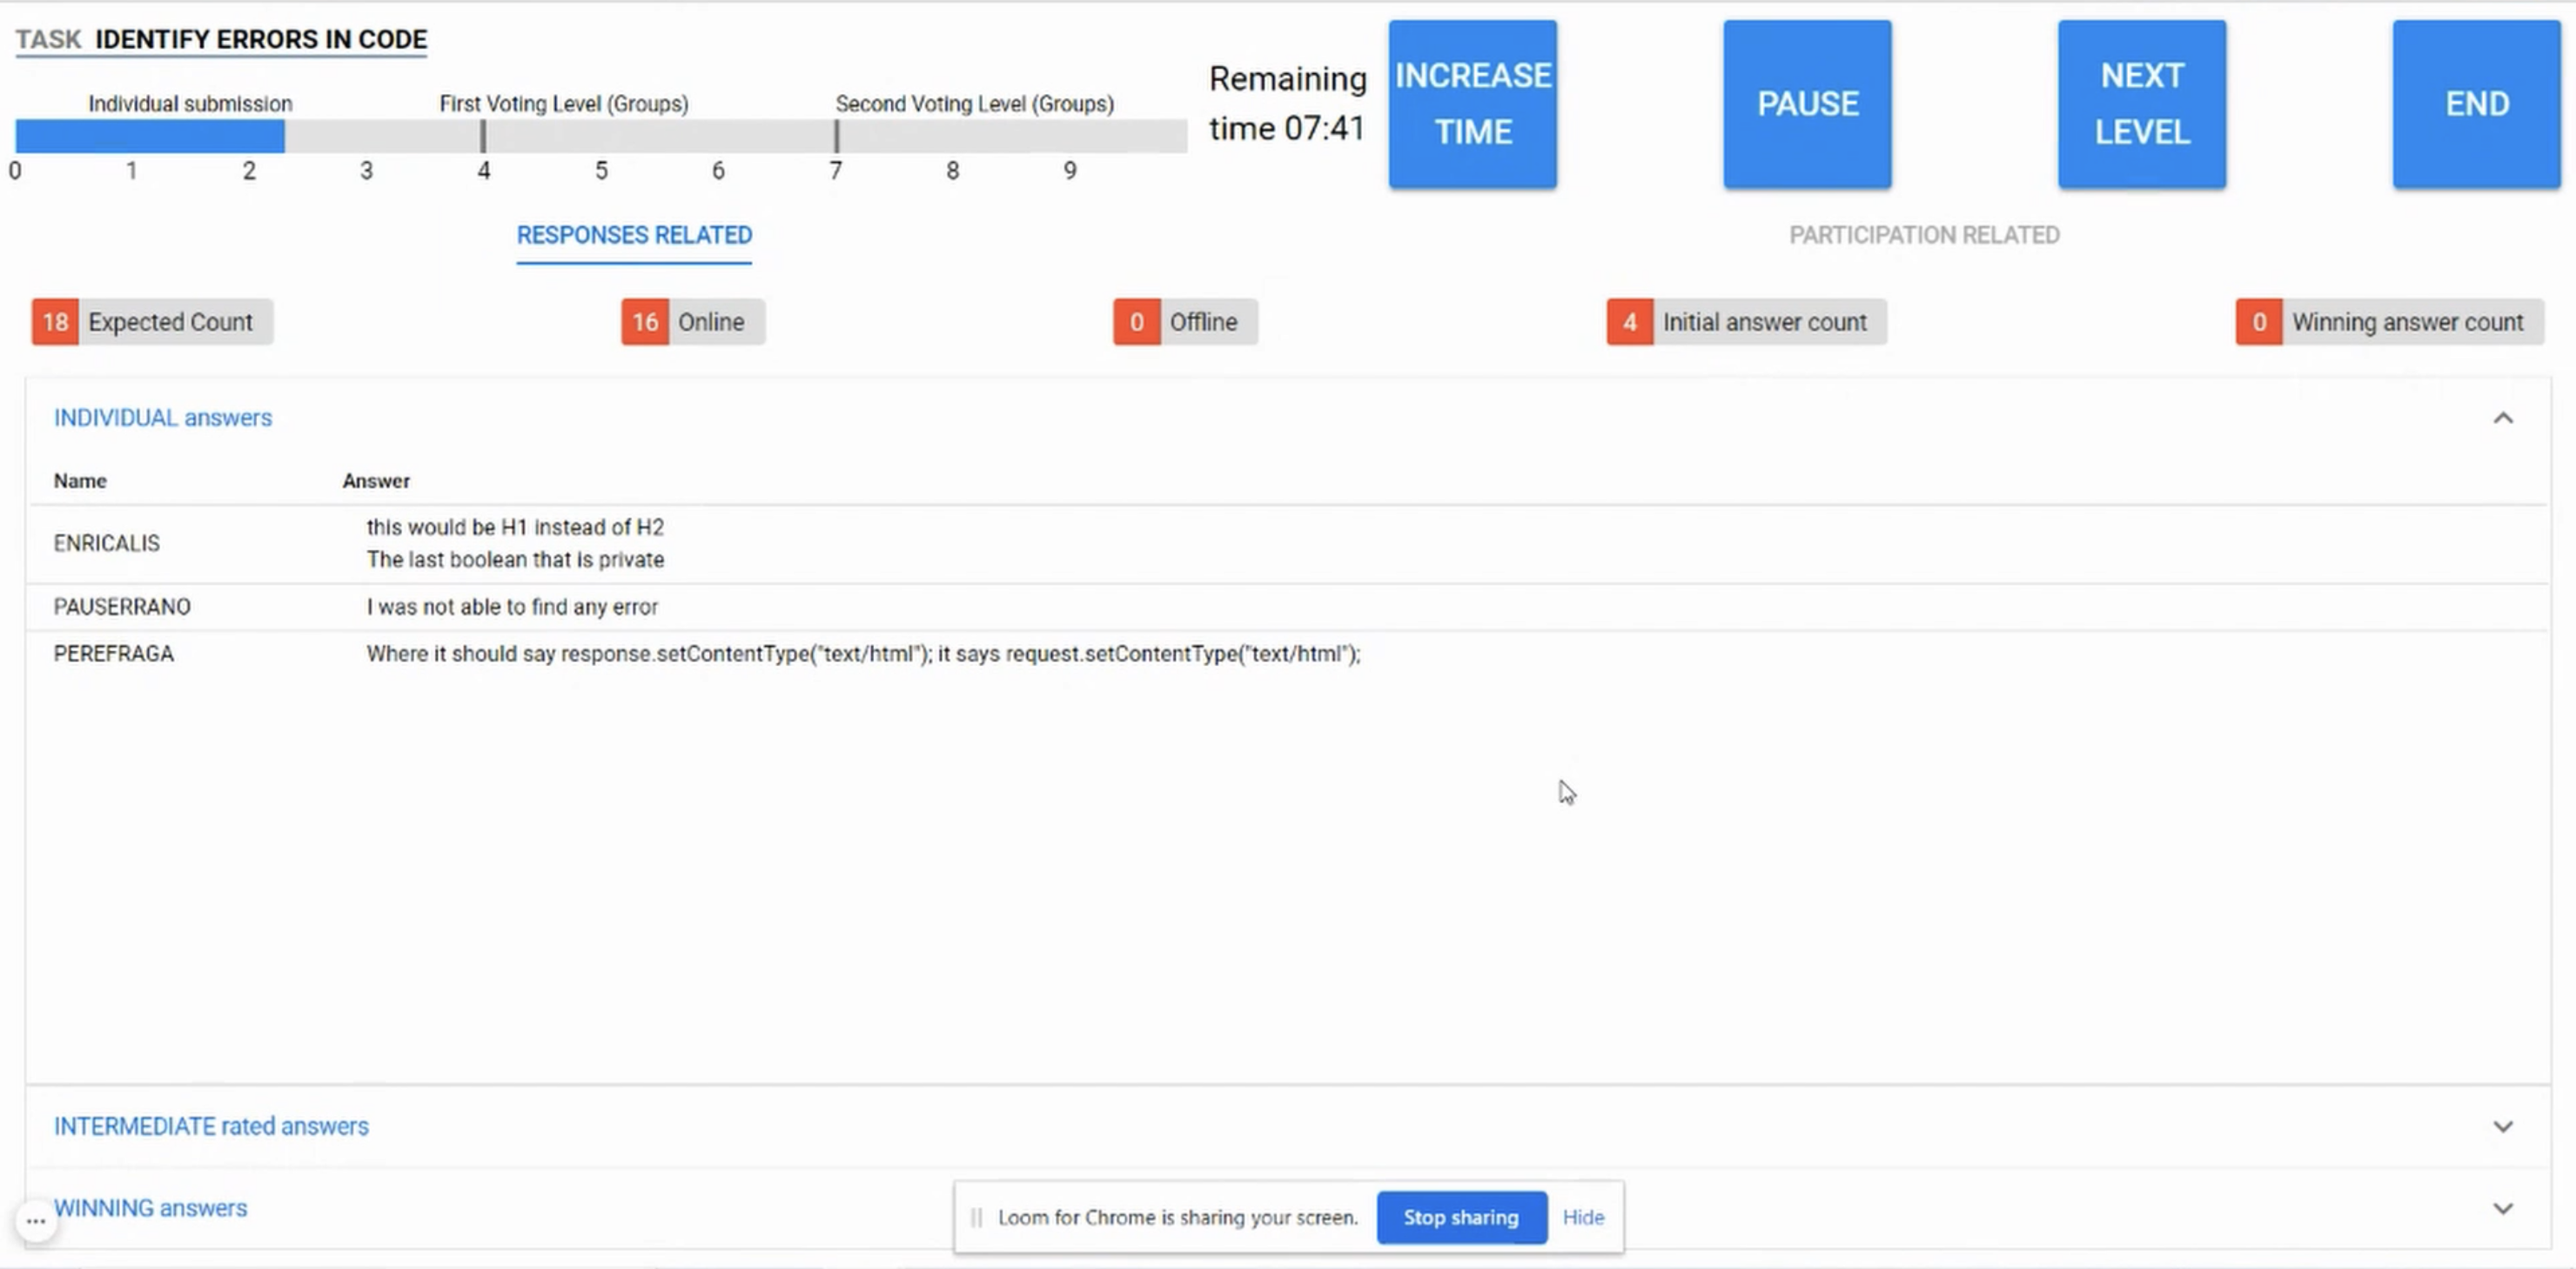
\includegraphics[clip,width=\columnwidth]{Figures/pyramidapp8.png}% 
\caption{Teacher-facing dashboard}
\label{fig:P8}
\end{figure}
\begin{figure}[!h]
    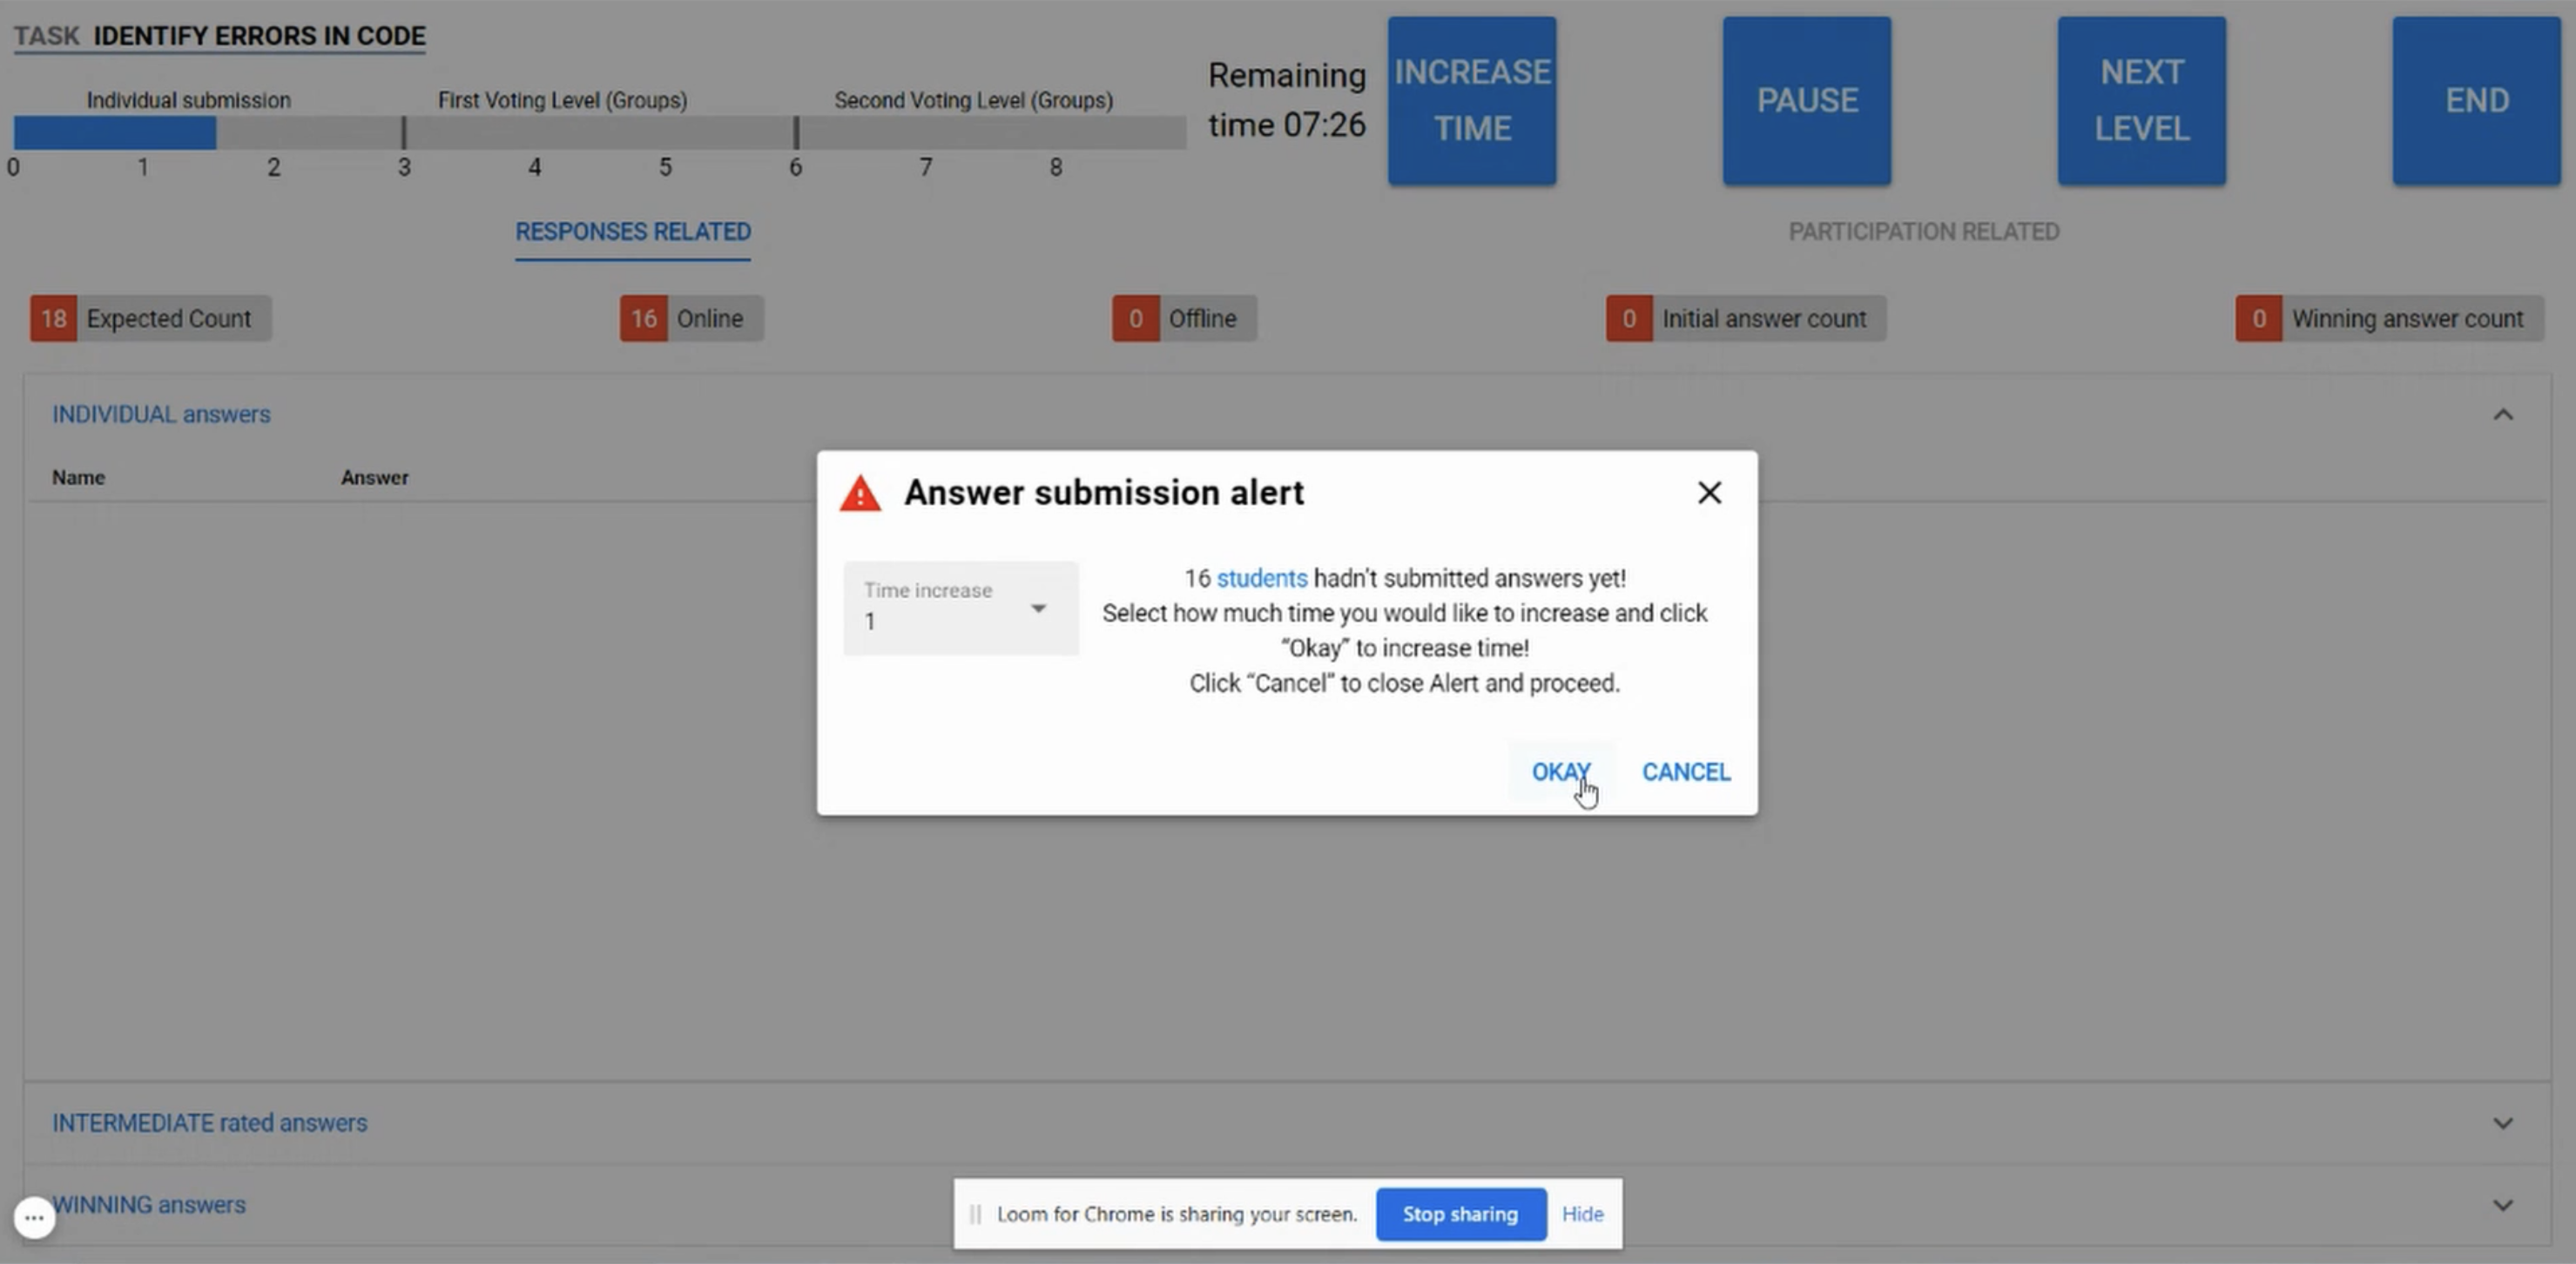
\includegraphics[clip,width=\columnwidth]{Figures/pyramidapp9.png}% 
\caption{Alert example}
\label{fig:P9}
\end{figure}
\begin{figure}[!h]
    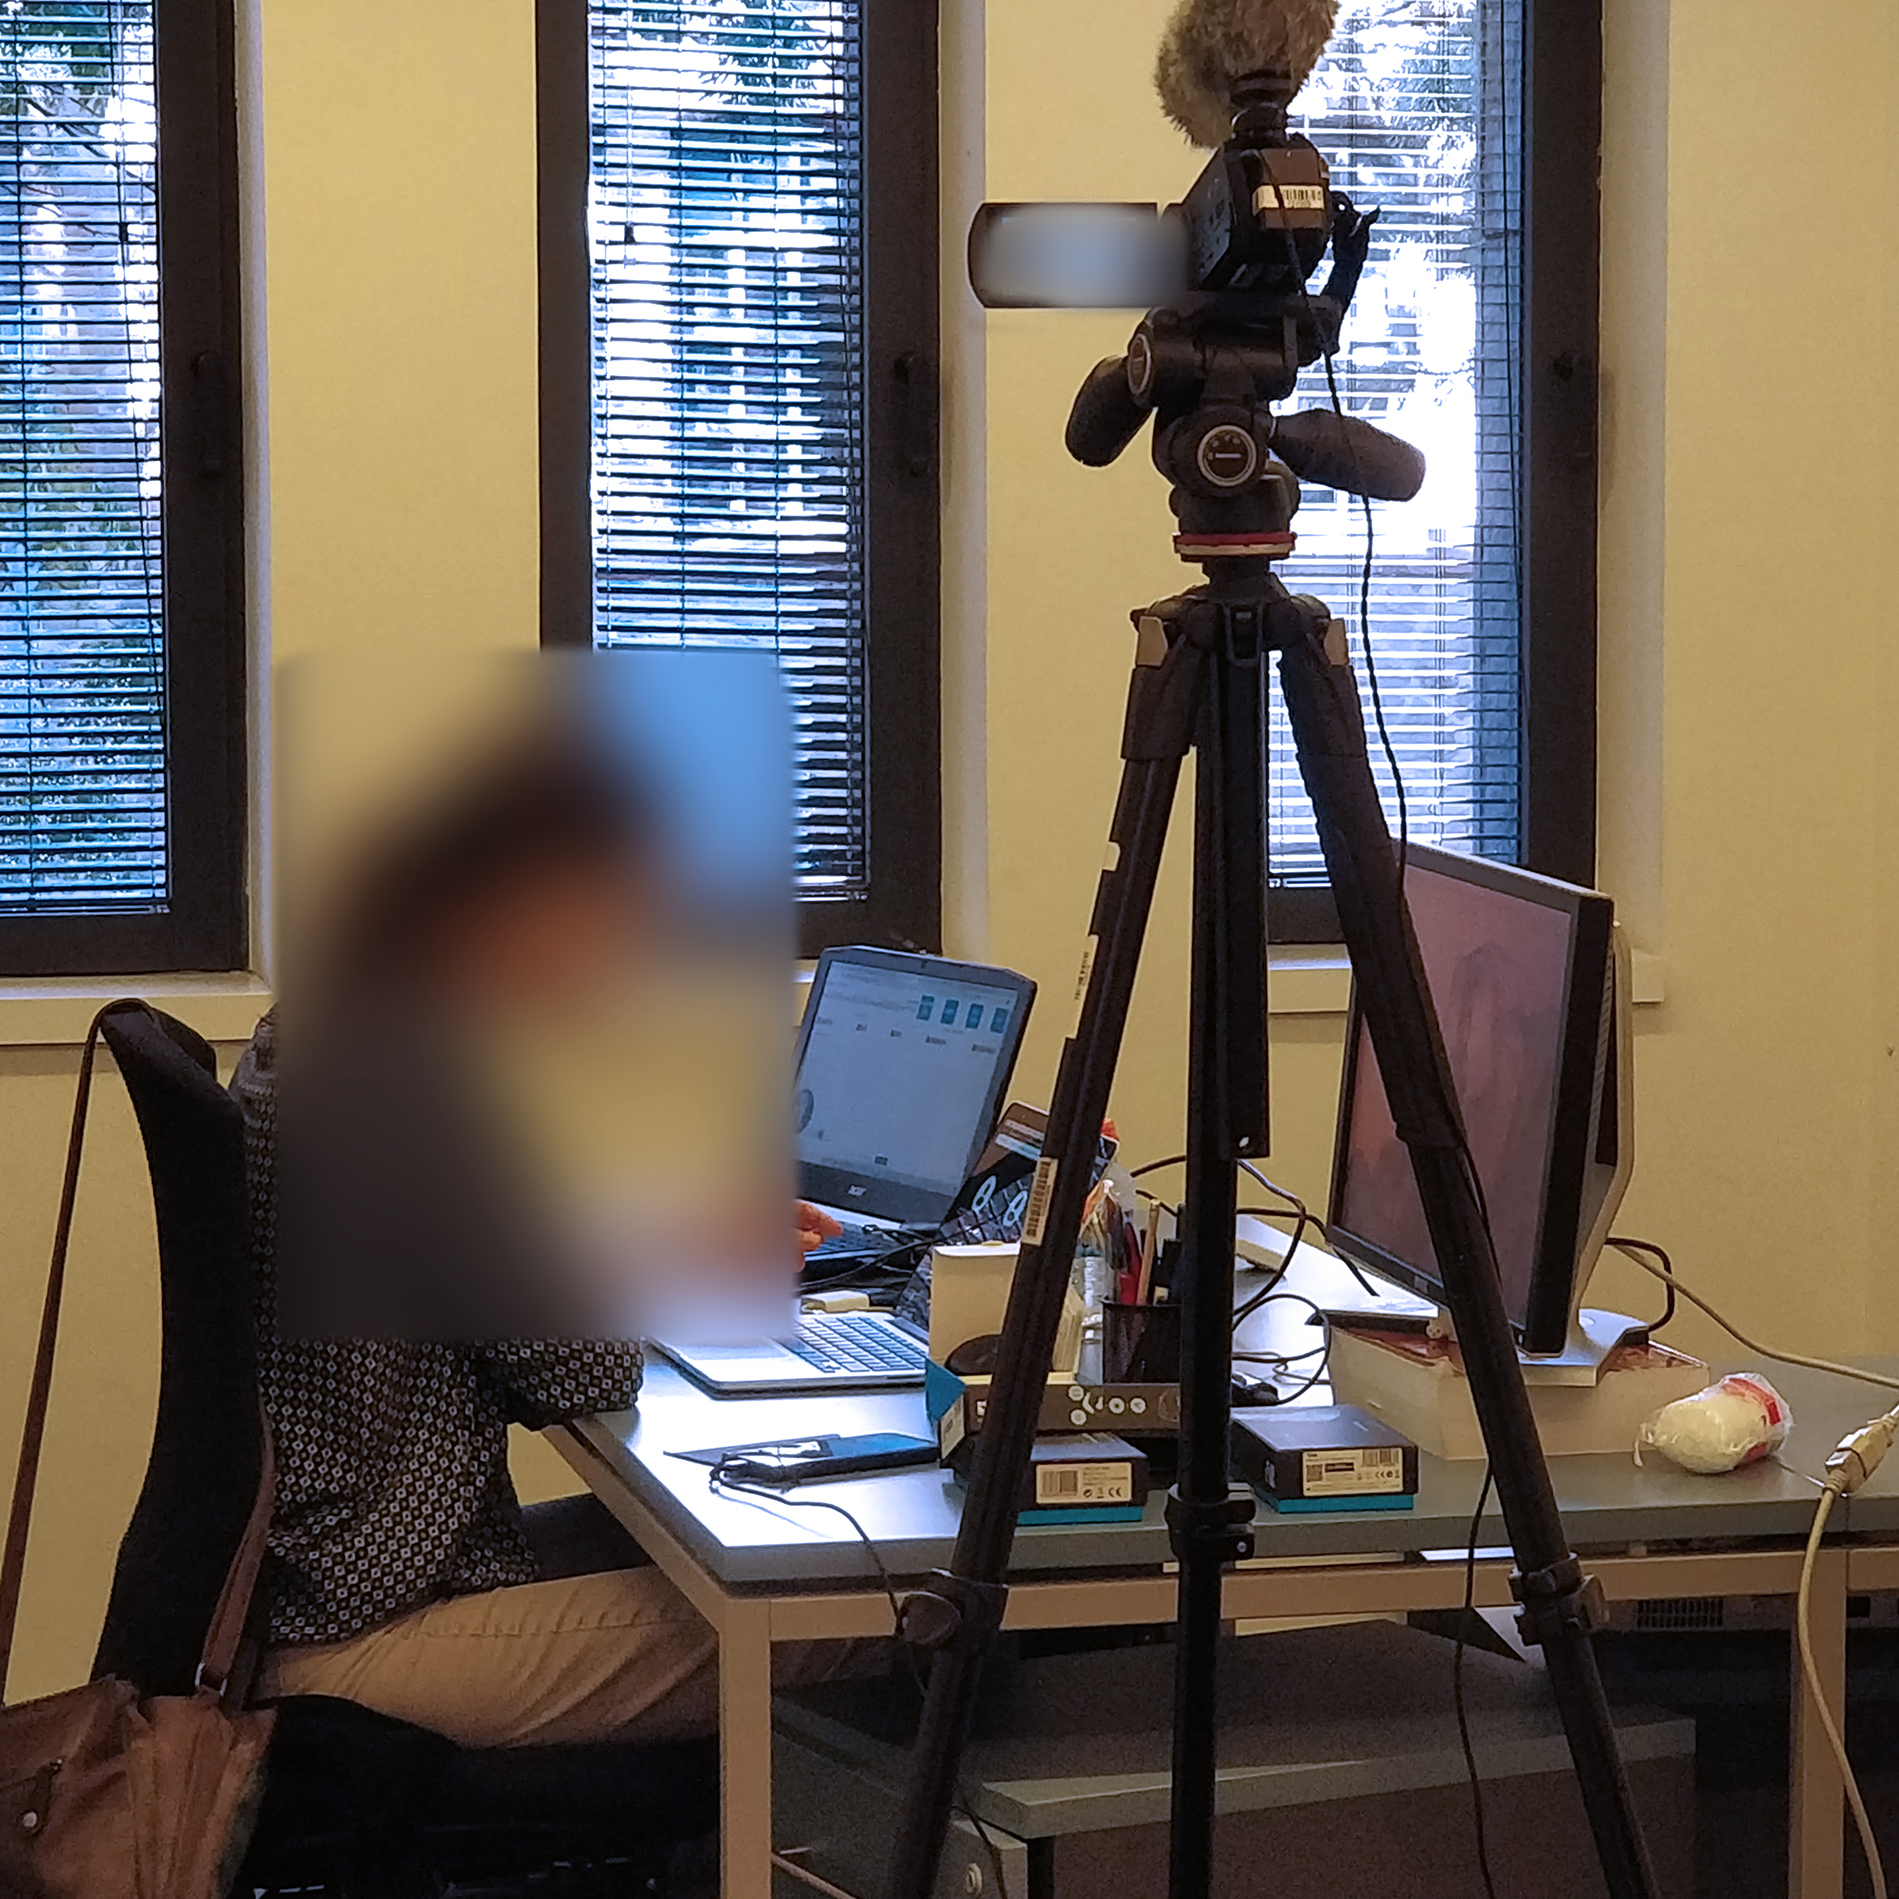
\includegraphics[clip,width=\textwidth]{Figures/environment.jpg}% 
\caption{Participant in the office}
\label{fig:environment} 
\end{figure}
\subsubsection{Electrodermal Activity}
Electrodermal activity was measured throughout the class, using a Shimmer3 electronic device with electrodes placed in the surface of the subject's skin (figure \ref{fig:shimmer}). The device was strapped to the subject's left forearm and the sensors were placed in the inner side of the left wrist. Wrists are an unobtrusive location for the electrodes, which are proven to have intermediate skin conductance responsiveness \cite{vandooren_de}.
\textbf{Hardware:} Consensys Shimmer3 GSR+
\textbf{Software:} ConsensysPRO software \cite{shimmer}
For each session, the researcher started the recording before the class began, and registered the time. After the session was over, the recording was stopped, time was registered again and data was stored.
\begin{figure}[!h]
    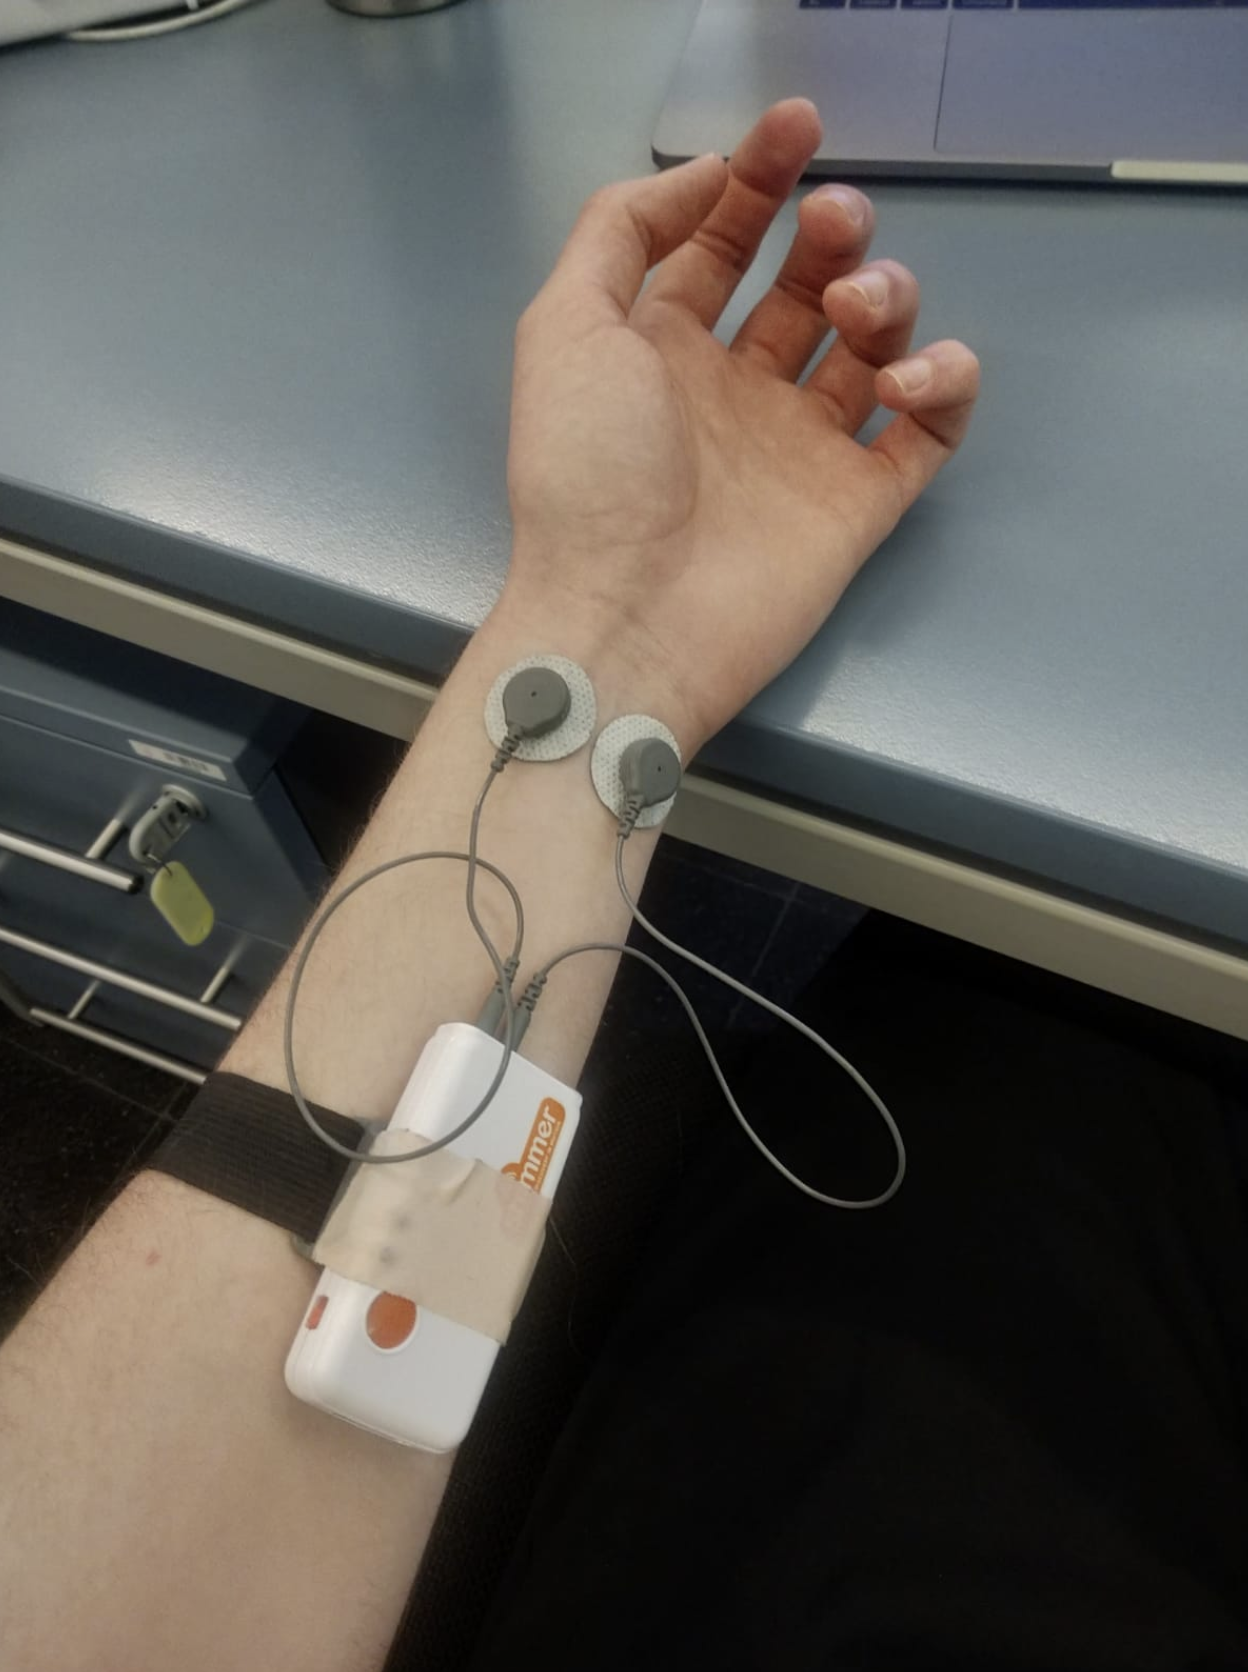
\includegraphics[clip,width=\columnwidth]{Figures/shimmer.png}% 
\caption{Participant in the office}
\label{fig:shimmer}
\end{figure}
\subsubsection{Post-activity questionnaire}
\textbf{Software:} Google Forms, Google Sheet.
After each session, when all sensors were removed, teachers were asked to fill a post-activity questionnaire. The questionnaire was designed for the participant to reflect on the session and to write down stressful moments they might have experienced. Data was stored using Google Sheets. (Appendix A)
\subsection{Procedure for usability evaluation data collection}
Similar to the recruitment of participants for the orchestration load measurements, a purposive sampling approach was taken to recruit a sample of 6/8 evaluators to analyse the usability of the teacher-facing dashboard that teachers used in each session. As done by Nielsen \cite{Nielsen1994-un}, evaluators were classified as usability specialists, CSCL specialists or double specialists (people who had combined experience in both). Usability specialists were defined as people that had already done usability inspections in a research or industry context before participating in this project. CSCL specialists were defined as people that had previous experience authoring and moderating classes using CSCL software.\\
Usability specialists that had no previous experience with PyramidApp were introduced to the tool. CSCL specialists that had no previous experience with Usability Heuristics were introduced to the framework.\\
All specialists were provided with a set of materials that illustrated the usage of the teacher-facing dashboard in the context of PyramidApp tool (described in \ref{materials_usability}) and tasked to list usability problems detected in the software as it was used by the teachers in their classes. Evaluators were randomly assigned to the mirroring or guiding conditions. The list of problems detected by each evaluator was compiled into a master list (one master list per condition), in which duplicates were deleted. As done in Zhang, et al (2003)\cite{zhang_johnson_patel_paige_kubose_2003}, the master list was then sent to each evaluator, whom were tasked to rate each problem using a scale that ranged from 0 to 4 described in \ref{materials_usability}. The average rating of each problem was calculated. The output of this procedure is a list of all usability problems detected for each condition and the average severity rating for each problem.
\subsection{Materials for usability evaluation data collection} \label{materials_usability}
\subsubsection{Sourcing materials}
Potential evaluators were identified using the criteria described above and contacted by the researcher. An email template was written to contact potential evaluators in case it was necessary. Potential evaluators who expressed interest in participating, were sent a form to verify their expertise and classify them.
The sourcing form (\ref{appendix_usability-evaluation}) provided a brief description of the task that provided a notion of how much time and effort the usability evaluation would take. The form was sent digitally using Google Forms. 
\subsubsection{Description and instructions for the evaluation}
Once evaluators expressed interest in the project and were classified, they were presented with a document that described the evaluation procedure in detail. Evaluators were instructed to read this document before starting with the evaluation. This document consisted of an introduction to Pyramid CLFPs, a description with screenshots of PyramidApp, an anonymised video of a teacher using the dashboard and a description of each Usability Heuristic. The document contained a link to the next step, an evaluation table, described in the following section. A sample document is available in \ref{appendix_usability-evaluation}.
\subsubsection{Evaluation table}
A Google Sheet was created individually for each evaluator. The document contained a table with two columns. One column was used  to describe the problem detected, and the other column was used to write which heuristic was affected by that problem. For convenience of the evaluator, the sheet also provided the same description of the heuristics presented in the instructions for the evaluation. This way they would be able to easily check each heuristic as they reported usability problems in the teacher-facing dashboard.
\begin{figure}[!h]
    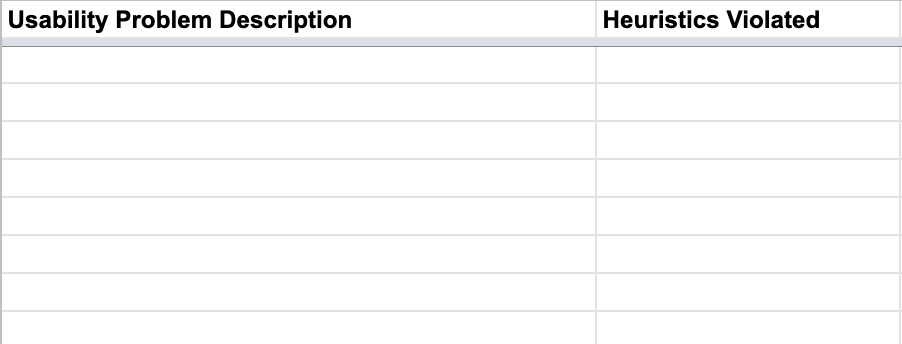
\includegraphics[clip,width=\columnwidth]{Figures/evaluation_table.png} 
\caption{Sample of usability evaluation table}
\label{fig:table-screenshot}
\end{figure}
\subsubsection{Master usability problems list}
After all evaluators were done reporting problems, all lists were inspected to compile a document with two master lists (one per condition) of all problems. Each list contained the problems reported by all evaluators. Duplicates were deleted so that the same problem wouldn't show twice. A copy of this list was sent to each evaluator.
All evaluators were instructed to rate the severity of each problem using a scale of 0-4. To frame the severity of each problem, they were presented with a scale of used by Zhang et al (2003) \cite{zhang_johnson_patel_paige_kubose_2003} as a reference:
\begin{itemize}
    \item \textbf{0}, not a usability problem at all
    \item \textbf{1}, cosmetic problem only. Need not be fixed unless extra time is available
    \item \textbf{2}, minor usability problem. Fixing this should be given low priority
    \item \textbf{3}, major usability problem. Important to fix. Should be given high priority
    \item \textbf{4}, usability catastrophe. Imperative to fix this before product is released
\end{itemize}
Ratings from all evaluators were averaged, resulting in two final documents with all usability problems detected and a severity rating for each problem.
\section{Data Analysis} \label{data-analysis}
All data collected was analysed to answer the research questions and address the initial hypotheses for each (described in \ref{research-questions}). As a common step towards answering both research questions, the self-perception questionnaires were inspected in search of possible changes in the affective state of the teacher. Then, the analysis branches for each research question, described as follows.
\subsection{Data analysis for research question 1}
\subsubsection{First analysis}
The following steps were taken for each condition:
\begin{itemize}
    \item Post activity questionnaires were inspected to look for the problems reported by the teacher.
    \item Screen recordings and video recordings were inspected to identify the precise moment in which problems described by the teachers in their post-activity questionnaires took place. The approximate time corresponding to each problem was noted.
    \item EDA information for each session was plotted in line charts. Using the time noted in the previous step, skin conductance was visually inspected to look for variances around the time of the problems reported by the teacher.
\end{itemize}
This analysis verified if and how many problems reported by the teacher are related to changes in skin conductance for each condition.
\subsubsection{Second Analysis}
The total amount of problems and the mean perceived cognitive load reported by the teacher for each condition were compared. This analysis outputted a number of problems that the teacher experienced for each condition, which makes both conditions comparable.
\subsubsection{Third Analysis}
EDA information for each session was averaged with the other session from the same condition. This analysis made the skin conductance measurements comparable for both conditions.
\subsection{Data analysis for research question 2}
The researcher will look for coincidences between the problems reported by the teacher and the problems in the master lists of usability problems. Since it will be known which problem reported by the teacher is related to a variance in their skin conductance, this step will output a qualitative analysis of the relationship between the problem experienced by the teacher, its variance in skin conductance and the problem reported by the specialists in Heuristic Evaluations.
\begin{figure}[!h]
    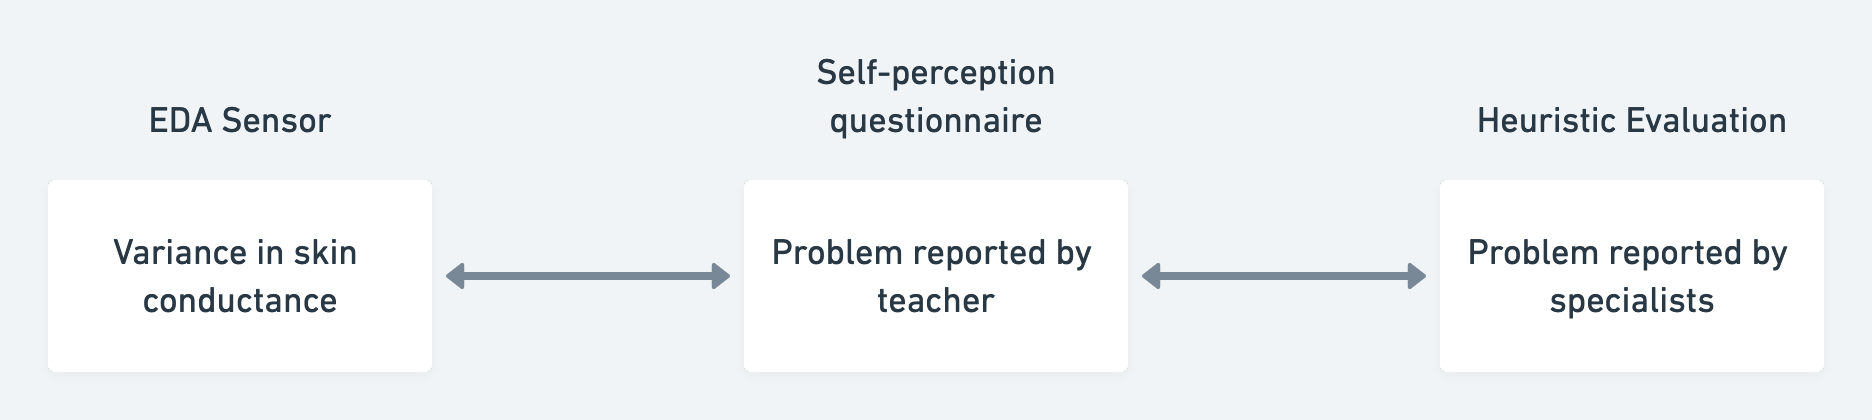
\includegraphics[clip,width=\columnwidth]{Figures/Heuristic-evaluation-diagram.png} 
\caption{Participant in the office} 
\label{fig:table}
\end{figure}
\section{Ethics}
Ethical considerations were taken for this project. Participants were not exposed to physical nor psychological harm or danger, collected data was stored securely and confidentially, and participants were fully informed of the procedures needed to perform the data collection before participating. Teachers who participated in the data collection were required to digitally complete and sign an informed consent form (\ref{appendix_consent}). This document contains the information of the principal researcher, supervisors and the institution that this research took place in. Through this document, teachers were presented with the motivation and duration of the research project, the research objectives, description of the methodologies and procedures, the name of the entities that have access to the data (namely UPF and TIDE), the risks associated with participating in the experiment, privacy and anonymity of the data, and the participants ability of withdrawing from the experiment without the need of justification.
\newpage


